\documentclass[12pt,a4paper]{report}

%-------------------- Packages ---------------------%
\usepackage[utf8]{inputenc}
\usepackage[T1]{fontenc}
\usepackage[french]{babel}

% Helvetica Font Family
\usepackage{helvet}
\renewcommand{\familydefault}{\sfdefault}

\usepackage{tikz}
\usetikzlibrary{shapes,arrows,positioning,fit}
\usepackage[top=2.5cm,bottom=2.5cm,right=2cm,left=2.5cm]{geometry}
\usepackage{graphicx}
\usepackage{hyperref}
\usepackage{xcolor}
\usepackage{float}
\usepackage{array}
\usepackage{tabularx}
\usepackage{booktabs}
\usepackage{enumitem}
\usepackage{listings}
\usepackage{fancyhdr}
\usepackage{titlesec}
\usepackage{caption}
\usepackage{subcaption}
\usepackage{pdfpages}
\usepackage{tocloft}

%-------------------- Color Definitions ---------------------%
\definecolor{orangecustom}{RGB}{230,115,0}
\definecolor{bluecustom}{RGB}{0,51,102}
\definecolor{awsorange}{RGB}{255,153,0}
\definecolor{codegreen}{RGB}{0,128,0}
\definecolor{codegray}{RGB}{128,128,128}
\definecolor{codeblue}{RGB}{0,0,255}
\definecolor{backcolour}{RGB}{245,245,245}

%-------------------- Listings Configuration ---------------------%
\lstdefinestyle{mystyle}{
    backgroundcolor=\color{backcolour},
    commentstyle=\color{codegreen},
    keywordstyle=\color{codeblue},
    numberstyle=\tiny\color{codegray},
    stringstyle=\color{orangecustom},
    basicstyle=\ttfamily\small,
    breakatwhitespace=false,
    breaklines=true,
    captionpos=b,
    keepspaces=true,
    numbers=left,
    numbersep=5pt,
    showspaces=false,
    showstringspaces=false,
    showtabs=false,
    tabsize=2,
    frame=single,
    rulecolor=\color{codegray}
}
\lstset{style=mystyle}

%-------------------- Hyperref Configuration ---------------------%
\hypersetup{
    colorlinks=true,
    linkcolor=bluecustom,
    filecolor=magenta,
    urlcolor=awsorange,
    citecolor=bluecustom,
    pdftitle={Infrastructure Cloud de Supervision Centralisée sous AWS},
    pdfauthor={EL BADRY Mohammed},
}

%-------------------- Customizations ---------------------%
\setcounter{tocdepth}{3}
\setcounter{secnumdepth}{3}

\renewcommand{\tablename}{Tableau}
\renewcommand{\figurename}{Figure}
\renewcommand{\lstlistingname}{Code}

% Chapter title format
\titleformat{\chapter}[display]
{\normalfont\huge\bfseries\sffamily}{\chaptername\ \thechapter}{20pt}{\Huge}
\titlespacing*{\chapter}{0pt}{-20pt}{40pt}

%-------------------- Page Style ---------------------%
\pagestyle{fancy}
\fancyhf{}
\fancyhead[L]{\leftmark}
\fancyfoot[C]{\thepage}
\renewcommand{\headrulewidth}{0.4pt}

%-------------------- Document Start ---------------------%
\begin{document}

% ========== PAGE DE GARDE ==========
\pagestyle{empty}
% ============================================
% Page de Garde - Projet AWS Zabbix
% ============================================

\begin{titlepage}
\centering

% Logo ENSET

\includegraphics[width=0.85\textwidth]{images/logo-enset.png}

\vspace{1.2cm}

{\Large\bfseries DÉPARTEMENT MATHÉMATIQUES ET INFORMATIQUE}

\vspace{0.8cm}

{\large\bfseries Filière :}\\[0.3cm]
{\color{bluecustom}\large\bfseries «Big Data et Cloud Computing»}

\vspace{1cm}

{\color{black}\LARGE\bfseries Projet AWS Academy}

\vspace{0.8cm}

% Titre du projet dans un cadre
\begin{tikzpicture}
    \node[draw=orangecustom, rectangle, line width=2pt, inner sep=15pt, text width=0.85\textwidth, align=center] (box) {
        \color{black}\Large\textbf{Mise en œuvre d'une Infrastructure Cloud}\\[0.3cm]
        \color{black}\Large\textbf{de Supervision Centralisée sous AWS}\\[0.5cm]
        \color{bluecustom}\large Déploiement de Zabbix conteneurisé pour le monitoring\\d'un parc hybride (Linux \& Windows)
    };
\end{tikzpicture}

\vspace{1.2cm}

% Informations étudiant et encadrant
\begin{tikzpicture}
    \node[draw=orangecustom, rectangle, line width=1.5pt, inner sep=15pt, text width=0.85\textwidth, align=center] (box) {
        \begin{minipage}{0.45\textwidth}
            \centering
            \textbf{Réalisé par :}\\[0.4cm]
            EL BADRY Mohammed
        \end{minipage}
        \hfill
        \begin{minipage}{0.45\textwidth}
            \centering
            \textbf{Encadré par :}\\[0.4cm]
            Pr. Azeddine KHIAT
        \end{minipage}
    };
\end{tikzpicture}

\vspace{1cm}

% Technologies utilisées
\begin{tikzpicture}
    \node[draw=bluecustom, rectangle, rounded corners, line width=1pt, inner sep=10pt, text width=0.75\textwidth, align=center, fill=backcolour] {
        \small\textbf{Technologies :} AWS EC2 \textbullet{} Docker \textbullet{} Zabbix 7.0 \textbullet{} MySQL \textbullet{} Ubuntu \textbullet{} Windows Server
    };
\end{tikzpicture}

\vfill

% Année universitaire
{\large\bfseries Année Universitaire : 2025/2026}

\vspace{0.5cm}

% Footer

\includegraphics[width=0.9\textwidth]{images/footer.png}

\end{titlepage}
\newpage

% ========== TABLE DES MATIÈRES ==========
\pagenumbering{roman}
\tableofcontents
\clearpage

% ========== LISTE DES FIGURES ==========
\listoffigures
\clearpage

% ========== LISTE DES TABLEAUX ==========
\listoftables
\clearpage

% ========== CONTENU PRINCIPAL ==========
\pagenumbering{arabic}
\setcounter{page}{1}
\pagestyle{fancy}

% Chapitre 1 : Introduction
\chapter{Introduction}
\label{chap:introduction}

\section{Contexte Général}

L'analyse forensique des scènes de crime représente un domaine critique où la précision et la rapidité d'intervention peuvent avoir des conséquences significatives sur le cours d'une enquête. Traditionnellement, cette analyse repose sur l'expertise humaine, ce qui peut être sujet à des erreurs, des biais ou des limitations temporelles.

L'avènement de l'intelligence artificielle et du Deep Learning offre de nouvelles perspectives pour augmenter les capacités des experts forensiques. Les techniques de vision par ordinateur permettent désormais de détecter automatiquement des objets d'intérêt, d'extraire des informations textuelles et de générer des hypothèses préliminaires.

Notre projet, \textbf{AI Forensic Avatar}, s'inscrit dans cette démarche d'innovation en proposant un système complet d'analyse forensique assistée par l'IA, doté d'une interface utilisateur immersive basée sur un avatar 3D interactif.

\section{Problématique}

L'analyse de scènes de crime présente plusieurs défis majeurs :

\begin{enumerate}
    \item \textbf{Volume de données} : Les enquêtes modernes génèrent un nombre considérable d'images et de preuves visuelles qui nécessitent un traitement rapide.
    
    \item \textbf{Expertise limitée} : Les experts forensiques qualifiés sont rares et leur temps est précieux.
    
    \item \textbf{Subjectivité} : L'interprétation humaine peut varier d'un expert à l'autre, introduisant des biais potentiels.
    
    \item \textbf{Accessibilité} : Les outils d'analyse professionnels sont souvent coûteux et complexes à utiliser.
    
    \item \textbf{Communication} : La présentation des résultats d'analyse peut être technique et difficile à comprendre pour les non-spécialistes.
\end{enumerate}

\section{Objectifs du Projet}

Notre projet vise à développer une solution logicielle complète répondant aux objectifs suivants :

\subsection{Objectifs Techniques}

\begin{itemize}
    \item Implémenter un pipeline d'analyse d'images utilisant des modèles de Deep Learning état de l'art
    \item Développer une API REST robuste et performante avec FastAPI
    \item Créer une interface utilisateur moderne et intuitive avec React et Three.js
    \item Intégrer un système de streaming en temps réel pour les réponses de l'IA
    \item Mettre en place un avatar 3D avec synchronisation labiale pour une expérience immersive
\end{itemize}

\subsection{Objectifs Fonctionnels}

\begin{itemize}
    \item Permettre le téléchargement et l'analyse automatique d'images de scènes
    \item Détecter et classifier les objets présents sur les images
    \item Extraire le texte visible (plaques d'immatriculation, panneaux, documents)
    \item Générer des hypothèses forensiques basées sur les preuves détectées
    \item Offrir une interface conversationnelle avec l'avatar pour discuter des analyses
\end{itemize}

\section{Technologies Utilisées}

Le tableau \ref{tab:technologies} présente les principales technologies utilisées dans ce projet :

\begin{table}[H]
\centering

\label{tab:technologies}
\begin{tabular}{@{}llp{9cm}@{}}
\toprule
\textbf{Catégorie} & \textbf{Technologie} & \textbf{Rôle} \\
\midrule
\multirow{4}{*}{Backend} 
    & FastAPI & Framework web Python asynchrone \\
    & PostgreSQL & Base de données relationnelle \\
    & MinIO & Stockage objet compatible S3 \\
    & SQLAlchemy & ORM pour Python \\
\midrule
\multirow{4}{*}{IA/ML}
    & YOLOv8 & Détection d'objets en temps réel \\
    & Tesseract & Reconnaissance optique de caractères \\
    & Ollama/OpenAI & Génération de texte (LLM) \\
    & Groq PlayAI & Synthèse vocale (TTS) \\
\midrule
\multirow{4}{*}{Frontend}
    & React 19 & Bibliothèque UI JavaScript \\
    & Three.js & Rendu 3D WebGL \\
    & React Three Fiber & Intégration Three.js avec React \\
    & Zustand & Gestion d'état \\
\midrule
\multirow{2}{*}{DevOps}
    & Docker & Conteneurisation \\
    & Docker Compose & Orchestration multi-conteneurs \\
\bottomrule
\end{tabular}
\caption{Stack Technologique du Projet}
\end{table}

\section{Organisation du Rapport}

Ce rapport est organisé comme suit :

\begin{description}
    \item[Chapitre 2 - État de l'Art] Présente les concepts théoriques et les technologies existantes dans les domaines de la vision par ordinateur, du traitement du langage naturel et des interfaces 3D.
    
    \item[Chapitre 3 - Architecture Système] Décrit l'architecture globale du système, les choix de conception et les patterns utilisés.
    
    \item[Chapitre 4 - Implémentation Backend] Détaille l'implémentation du serveur FastAPI, les services IA et la gestion des données.
    
    \item[Chapitre 5 - Implémentation Frontend] Présente le développement de l'interface utilisateur React et l'intégration de l'avatar 3D.
    
    \item[Chapitre 8 - Conclusion] Résume les contributions et propose des perspectives d'amélioration.
\end{description}

% ============================================
% Chapitre 2 : Architecture Réseau
% ============================================
\chapter{Architecture Réseau}
\label{chap:architecture}

\section{Vue d'Ensemble}

L'architecture réseau déployée sur AWS repose sur un Virtual Private Cloud (VPC) configuré pour héberger l'ensemble de l'infrastructure de monitoring. Cette architecture a été conçue en tenant compte des limitations du Learner Lab AWS Academy.

\section{Schéma d'Architecture}

\begin{figure}[H]
\centering
\begin{tikzpicture}[
    node distance=1.5cm,
    box/.style={rectangle, draw=bluecustom, line width=1.5pt, minimum width=3cm, minimum height=1.2cm, align=center, font=\small},
    cloud/.style={rectangle, draw=awsorange, line width=2pt, minimum width=12cm, minimum height=8cm, align=center, rounded corners},
    subnet/.style={rectangle, draw=codegreen, line width=1pt, minimum width=11cm, minimum height=5.5cm, align=center, dashed}
]

% VPC
\node[cloud, label={[font=\bfseries]above:AWS VPC (10.0.0.0/16)}] (vpc) {};

% Subnet
\node[subnet, label={[font=\small]above:Subnet Public (10.0.1.0/24)}] at (0,-0.5) (subnet) {};

% Instances
\node[box, fill=awsorange!20] at (-4,-0.5) (zabbix) {Zabbix Server\\t3.large\\10.0.1.x};
\node[box, fill=codegreen!20] at (0,-0.5) (linux) {Client Linux\\t3.medium\\10.0.1.x};
\node[box, fill=codeblue!20] at (4,-0.5) (windows) {Client Windows\\t3.large\\10.0.1.x};

% Internet Gateway
\node[box, fill=awsorange!40] at (0,-4.5) (igw) {Internet Gateway};

% Internet
\node[box, fill=gray!20] at (0,-6.5) (internet) {Internet};

% Connections
\draw[->, thick] (igw) -- (internet);
\draw[->, thick] (subnet.south) -- (igw);

\end{tikzpicture}
\caption{Architecture réseau du projet AWS Zabbix}
\label{fig:architecture}
\end{figure}

\section{Création du VPC}

\subsection{Configuration du VPC}

Le VPC a été créé avec les paramètres suivants :

\begin{table}[H]
\centering
\caption{Configuration du VPC}
\label{tab:vpc-config}
\begin{tabular}{|l|l|}
\hline
\textbf{Paramètre} & \textbf{Valeur} \\
\hline
Nom & ELBadry-Zabbix-VPC \\
\hline
IPv4 CIDR & 10.0.0.0/16 \\
\hline
IPv6 & Désactivé \\
\hline
Tenancy & Default \\
\hline
\end{tabular}
\end{table}

\begin{figure}[H]
\centering
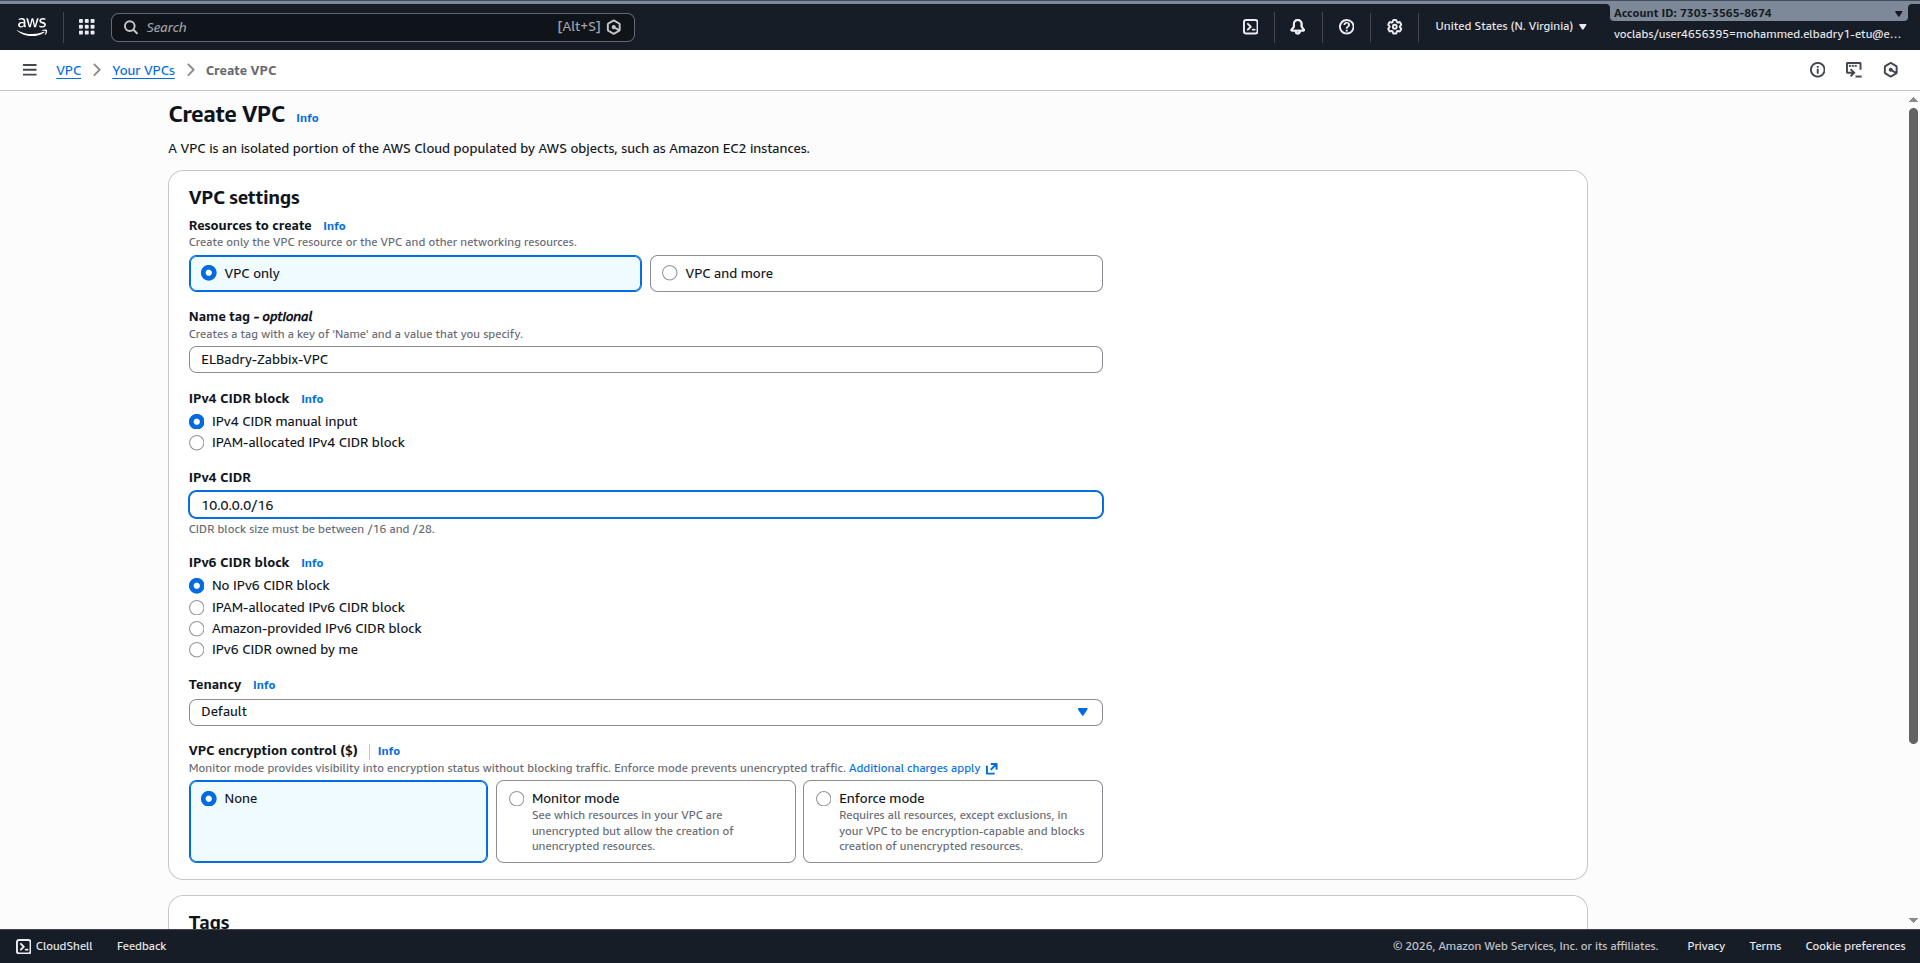
\includegraphics[width=0.9\textwidth]{images/01-vpc-creation.png}
\caption{Création du VPC dans la console AWS}
\label{fig:vpc-creation}
\end{figure}

\section{Configuration du Subnet}

\subsection{Subnet Public}

Un sous-réseau public a été créé pour héberger toutes les instances :

\begin{table}[H]
\centering
\caption{Configuration du Subnet}
\label{tab:subnet-config}
\begin{tabular}{|l|l|}
\hline
\textbf{Paramètre} & \textbf{Valeur} \\
\hline
Nom & ELBadry-Public-Subnet \\
\hline
VPC & ELBadry-Zabbix-VPC \\
\hline
Availability Zone & us-east-1a \\
\hline
IPv4 CIDR & 10.0.1.0/24 \\
\hline
Auto-assign Public IP & Activé \\
\hline
\end{tabular}
\end{table}

\begin{figure}[H]
\centering
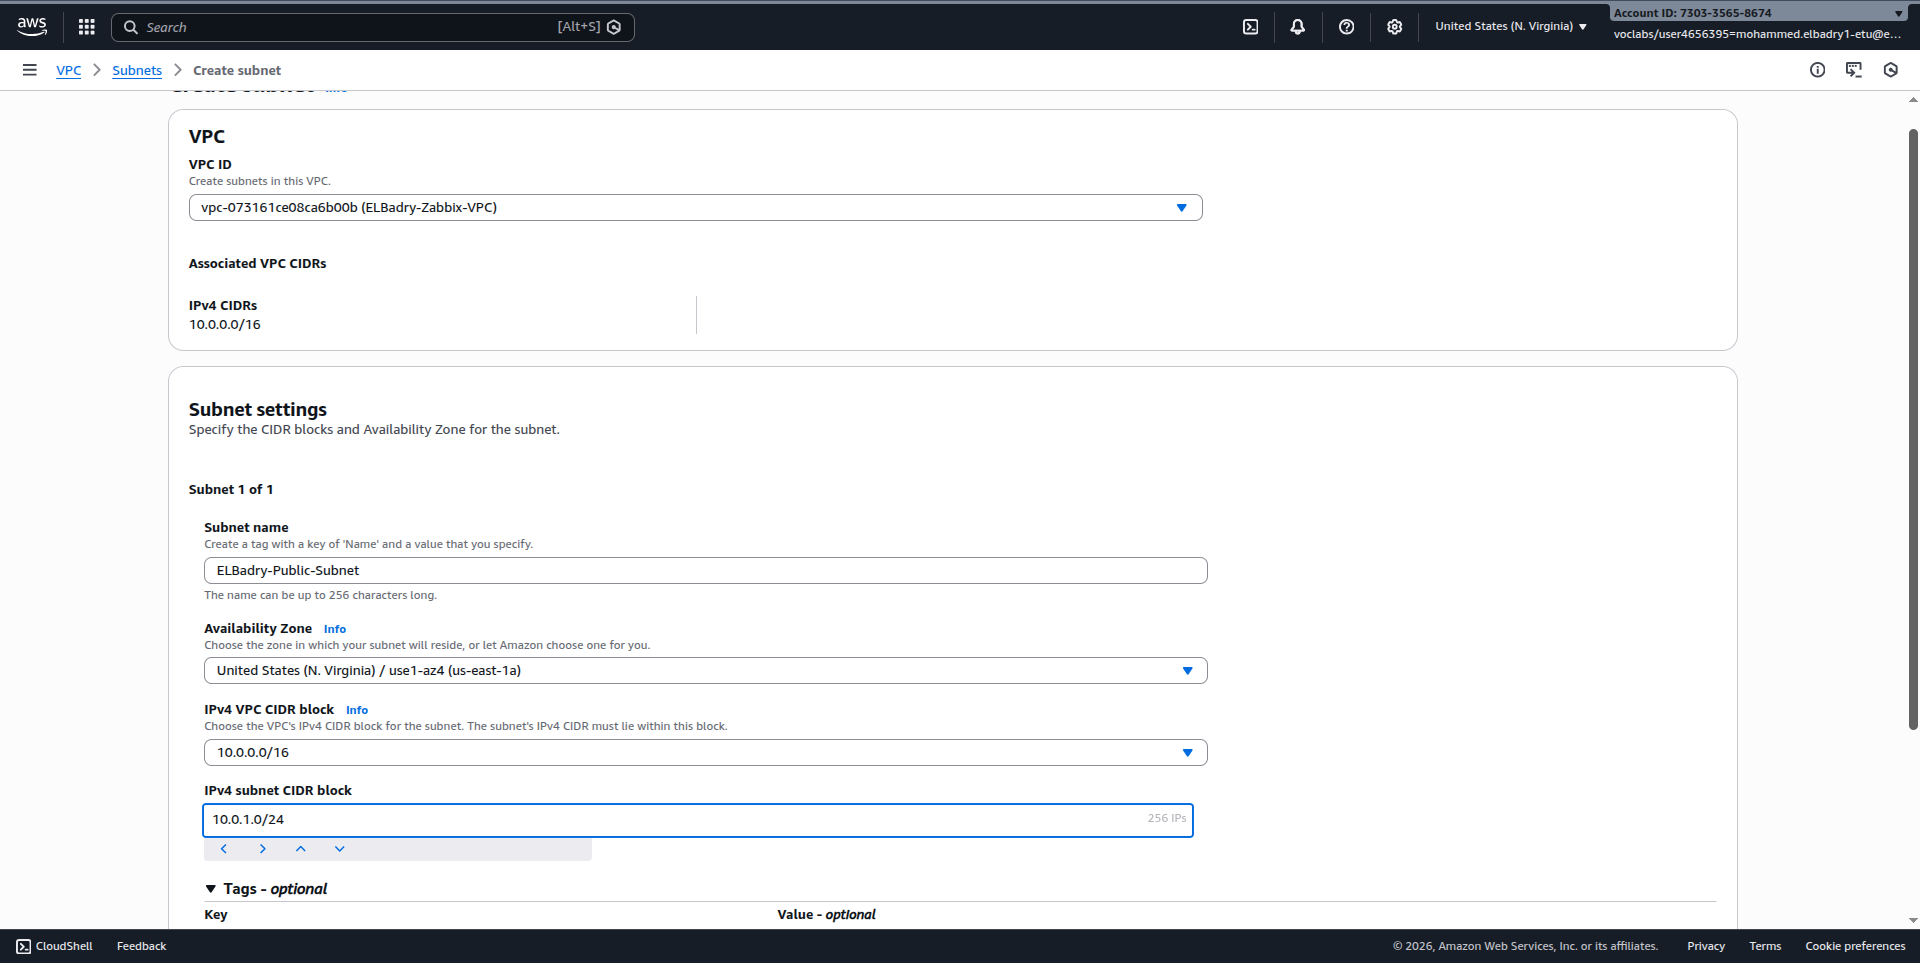
\includegraphics[width=0.9\textwidth]{images/02-subnet-configuration.png}
\caption{Configuration du Subnet public}
\label{fig:subnet-config}
\end{figure}

\section{Internet Gateway}

L'Internet Gateway permet aux instances du VPC de communiquer avec Internet :

\begin{enumerate}
    \item Création de l'Internet Gateway : \texttt{ELBadry-IGW}
    \item Attachement au VPC \texttt{ELBadry-Zabbix-VPC}
    \item Configuration de la table de routage avec la route \texttt{0.0.0.0/0} vers l'IGW
\end{enumerate}

\section{Security Groups}

\subsection{Security Group - Serveur Zabbix}

\begin{table}[H]
\centering
\caption{Règles du Security Group Zabbix Server}
\label{tab:sg-zabbix}
\begin{tabular}{|l|l|l|l|}
\hline
\textbf{Type} & \textbf{Port} & \textbf{Source} & \textbf{Description} \\
\hline
SSH & 22 & Mon IP & Accès SSH \\
\hline
HTTP & 80 & 0.0.0.0/0 & Interface Web Zabbix \\
\hline
HTTPS & 443 & 0.0.0.0/0 & Interface Web sécurisée \\
\hline
Custom TCP & 10050 & 10.0.0.0/16 & Zabbix Agent \\
\hline
Custom TCP & 10051 & 10.0.0.0/16 & Zabbix Trapper \\
\hline
\end{tabular}
\end{table}

\subsection{Security Group - Clients}

\begin{table}[H]
\centering
\caption{Règles du Security Group Clients}
\label{tab:sg-clients}
\begin{tabular}{|l|l|l|l|}
\hline
\textbf{Type} & \textbf{Port} & \textbf{Source} & \textbf{Description} \\
\hline
SSH & 22 & Mon IP & Accès SSH (Linux) \\
\hline
RDP & 3389 & Mon IP & Bureau à distance (Windows) \\
\hline
Custom TCP & 10050 & SG Zabbix Server & Agent Zabbix \\
\hline
\end{tabular}
\end{table}

\section{Tableau Récapitulatif des Ports}

\begin{table}[H]
\centering
\caption{Ports utilisés dans l'infrastructure}
\label{tab:ports}
\begin{tabular}{|l|l|p{7cm}|}
\hline
\textbf{Port} & \textbf{Service} & \textbf{Description} \\
\hline
22 & SSH & Accès sécurisé aux machines Linux \\
\hline
80 & HTTP & Interface Web Zabbix \\
\hline
443 & HTTPS & Interface Web Zabbix (sécurisé) \\
\hline
3389 & RDP & Bureau à distance Windows \\
\hline
10050 & Zabbix Agent & Communication passive (serveur → agent) \\
\hline
10051 & Zabbix Trapper & Communication active (agent → serveur) \\
\hline
\end{tabular}
\end{table}

% ============================================
% Chapitre 3 : Instances EC2
% ============================================
\chapter{Architecture des Instances EC2}
\label{chap:instances}

\section{Vue d'Ensemble des Instances}

Trois instances EC2 ont été déployées pour ce projet, chacune ayant un rôle spécifique dans l'infrastructure de monitoring.

\begin{table}[H]
\centering
\caption{Récapitulatif des instances EC2}
\label{tab:instances-summary}
\begin{tabular}{|l|l|l|l|}
\hline
\textbf{Instance} & \textbf{Type} & \textbf{OS} & \textbf{Rôle} \\
\hline
ELBadry-Zabbix-Server & t3.large & Ubuntu 22.04 & Serveur Zabbix (Docker) \\
\hline
ELBadry-Client-Linux & t3.medium & Ubuntu 22.04 & Client supervisé \\
\hline
ELBadry-Client-Windows & t3.large & Windows Server 2022 & Client supervisé \\
\hline
\end{tabular}
\end{table}

\begin{figure}[H]
\centering
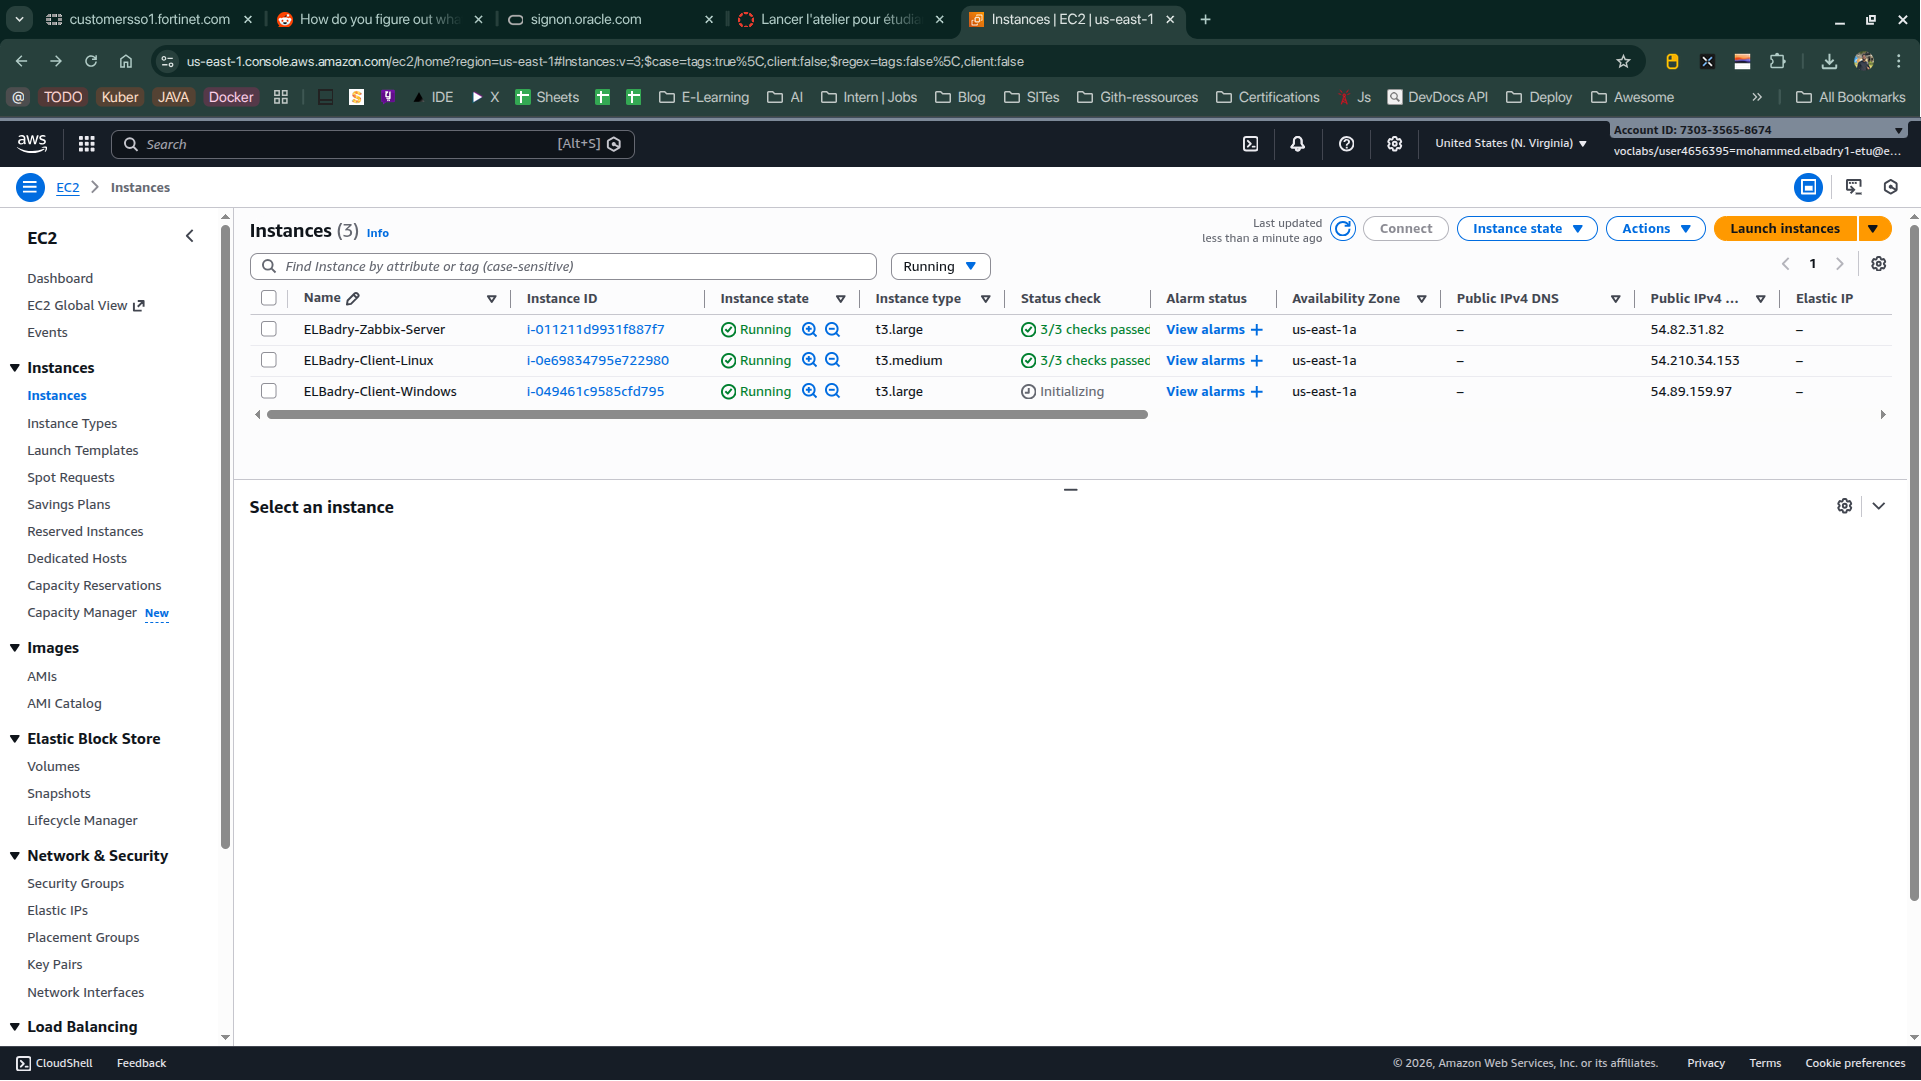
\includegraphics[width=0.95\textwidth]{images/03-instances-list-status.png}
\caption{Liste des instances EC2 en état Running}
\label{fig:instances-list}
\end{figure}

\section{Serveur Zabbix}

\subsection{Spécifications}

Le serveur Zabbix est le cœur de l'infrastructure de monitoring :

\begin{table}[H]
\centering
\caption{Configuration du serveur Zabbix}
\label{tab:zabbix-server-config}
\begin{tabular}{|l|l|}
\hline
\textbf{Paramètre} & \textbf{Valeur} \\
\hline
Nom & ELBadry-Zabbix-Server \\
\hline
Type d'instance & t3.large (2 vCPU, 8 Go RAM) \\
\hline
AMI & Ubuntu Server 22.04 LTS \\
\hline
Stockage & 30 Go gp3 \\
\hline
IP Privée & 10.0.1.x \\
\hline
Security Group & ELBadry-Zabbix-Server-SG \\
\hline
\end{tabular}
\end{table}

\begin{figure}[H]
\centering
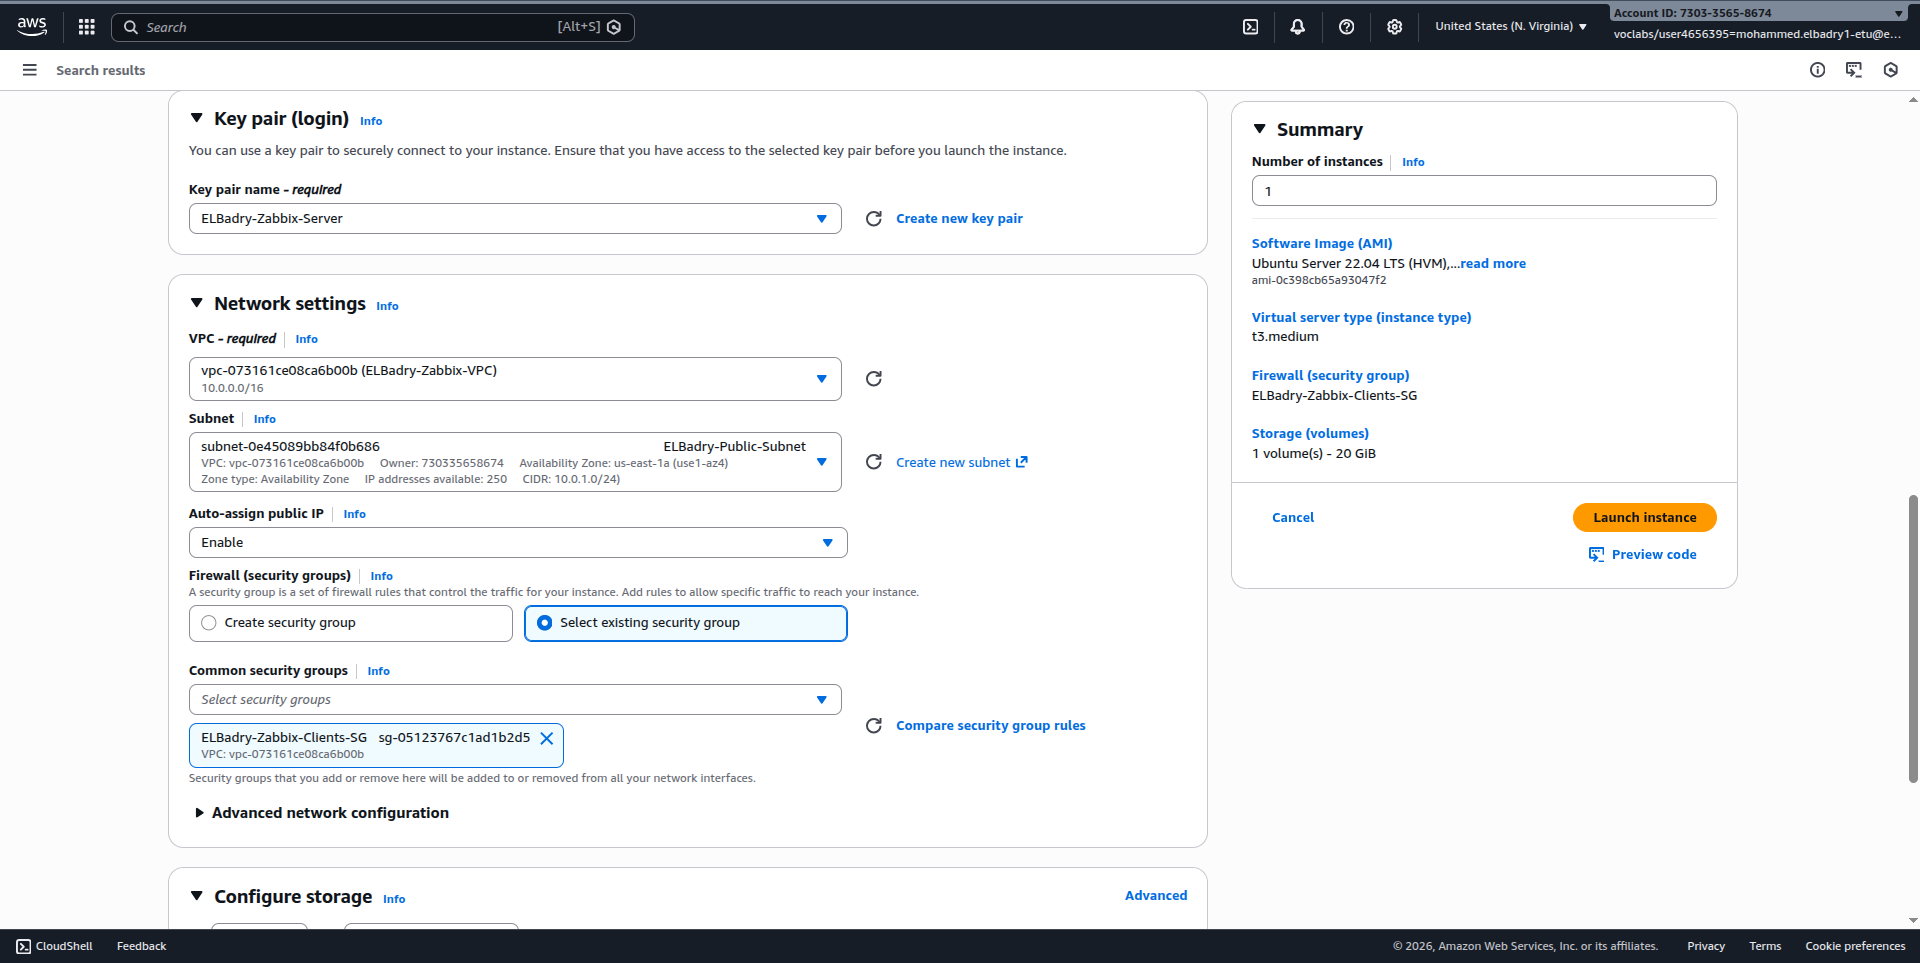
\includegraphics[width=0.95\textwidth]{images/05-instance-zabbix-server-details.png}
\caption{Détails de l'instance Zabbix Server}
\label{fig:zabbix-server-details}
\end{figure}

\subsection{Justification du Choix t3.large}

Le type t3.large a été choisi pour le serveur Zabbix car :
\begin{itemize}
    \item \textbf{8 Go de RAM} : Suffisant pour Docker, MySQL et Zabbix Server
    \item \textbf{2 vCPU} : Permet de gérer plusieurs conteneurs simultanément
    \item \textbf{Performances en rafale} : Adapté aux pics de charge
    \item \textbf{Compatible Learner Lab} : Type d'instance autorisé
\end{itemize}

\section{Client Linux}

\subsection{Spécifications}

\begin{table}[H]
\centering
\caption{Configuration du client Linux}
\label{tab:client-linux-config}
\begin{tabular}{|l|l|}
\hline
\textbf{Paramètre} & \textbf{Valeur} \\
\hline
Nom & ELBadry-Client-Linux \\
\hline
Type d'instance & t3.medium (2 vCPU, 4 Go RAM) \\
\hline
AMI & Ubuntu Server 22.04 LTS \\
\hline
Stockage & 20 Go gp3 \\
\hline
IP Privée & 10.0.1.x \\
\hline
Security Group & ELBadry-Zabbix-Clients-SG \\
\hline
\end{tabular}
\end{table}

\begin{figure}[H]
\centering
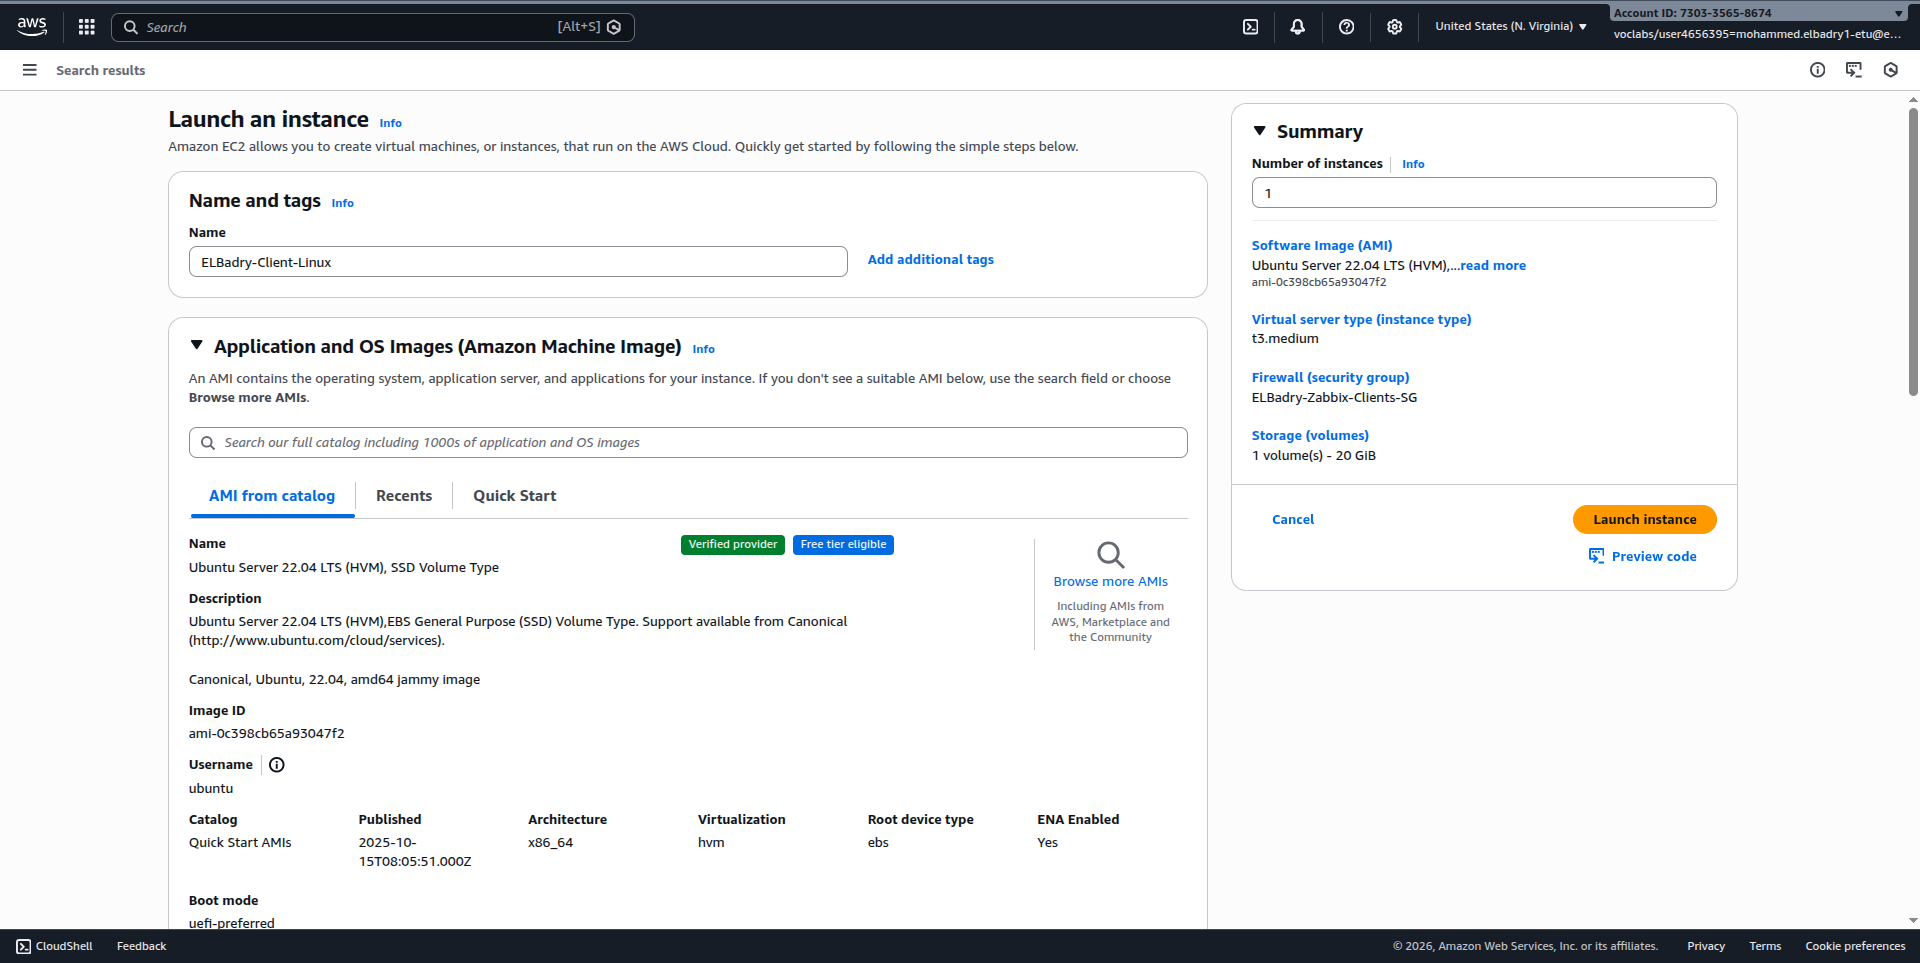
\includegraphics[width=0.95\textwidth]{images/10-instance-client-linux-details.png}
\caption{Détails de l'instance Client Linux}
\label{fig:client-linux-details}
\end{figure}

\section{Client Windows}

\subsection{Spécifications}

\begin{table}[H]
\centering
\caption{Configuration du client Windows}
\label{tab:client-windows-config}
\begin{tabular}{|l|l|}
\hline
\textbf{Paramètre} & \textbf{Valeur} \\
\hline
Nom & ELBadry-Client-Windows \\
\hline
Type d'instance & t3.large (2 vCPU, 8 Go RAM) \\
\hline
AMI & Microsoft Windows Server 2022 Base \\
\hline
Stockage & 30 Go gp3 \\
\hline
IP Privée & 10.0.1.x \\
\hline
Security Group & ELBadry-Zabbix-Clients-SG \\
\hline
\end{tabular}
\end{table}

\begin{figure}[H]
\centering
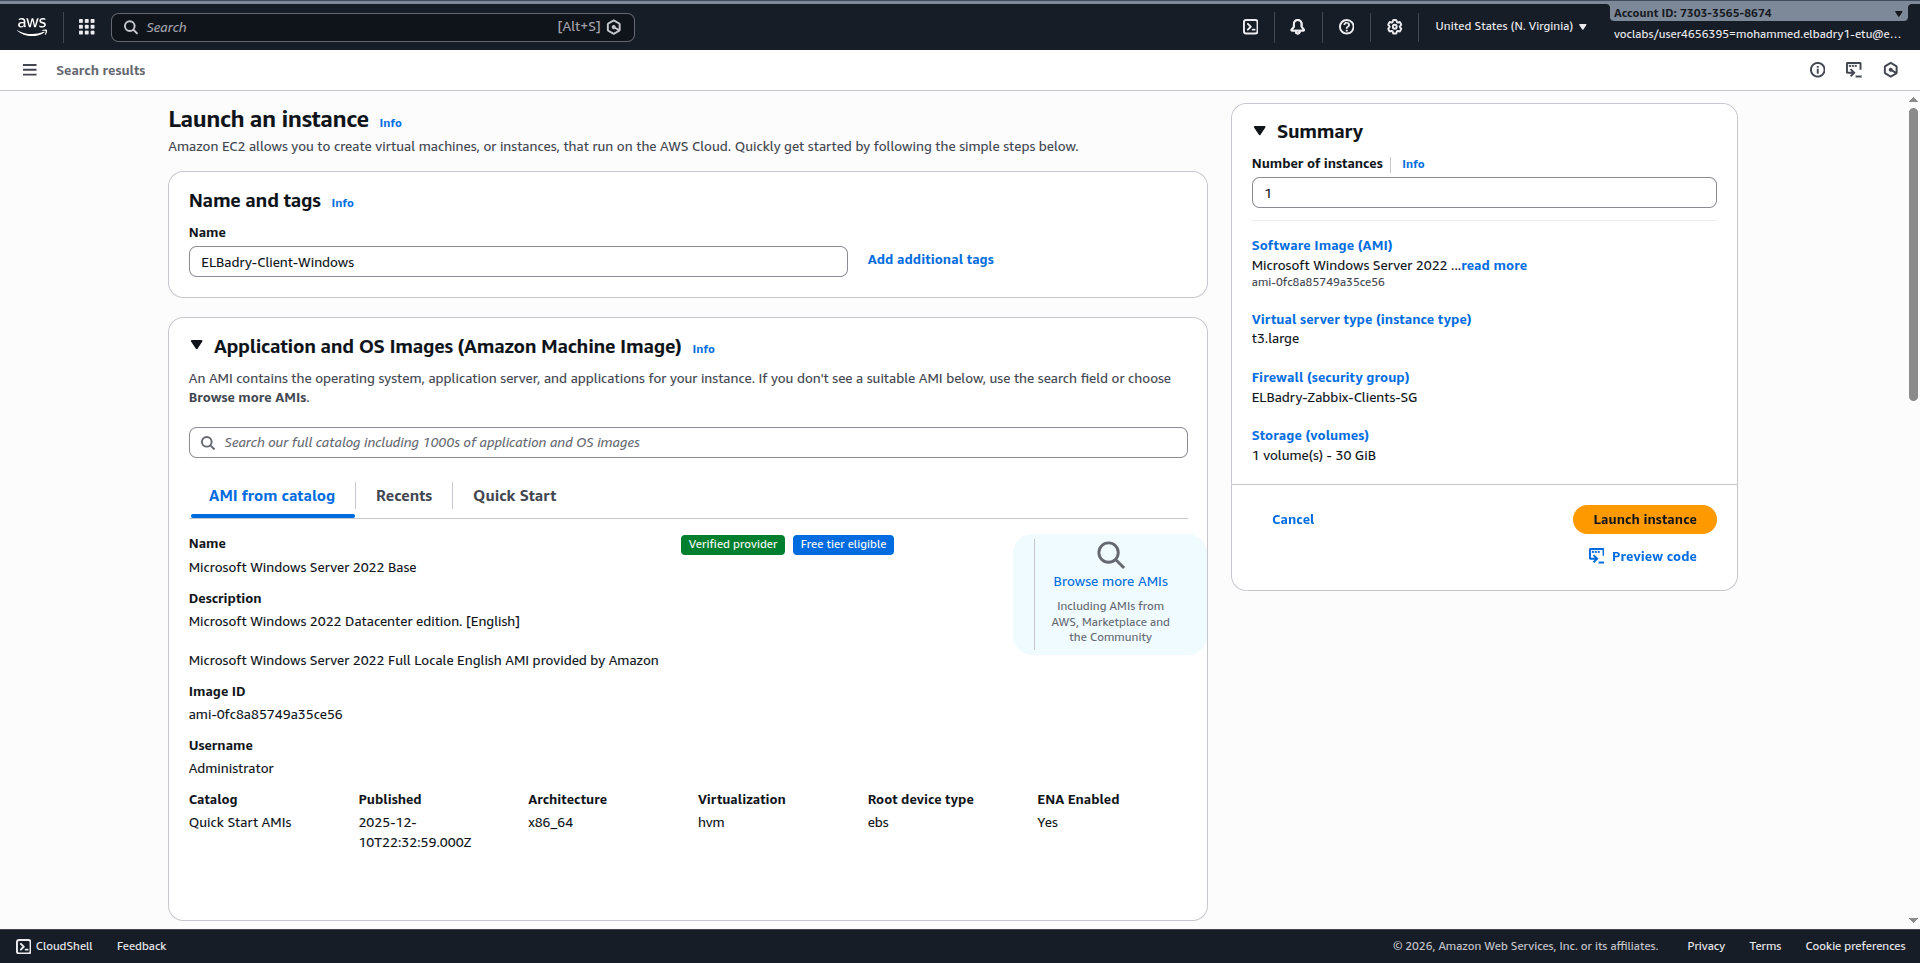
\includegraphics[width=0.95\textwidth]{images/11-instance-client-windows-details.png}
\caption{Détails de l'instance Client Windows}
\label{fig:client-windows-details}
\end{figure}

\subsection{Récupération du Mot de Passe Windows}

Pour accéder au client Windows via RDP, il est nécessaire de récupérer le mot de passe administrateur :

\begin{enumerate}
    \item Sélectionner l'instance Windows
    \item Actions → Security → Get Windows Password
    \item Charger la clé privée (.pem)
    \item Déchiffrer le mot de passe
\end{enumerate}

\begin{figure}[H]
\centering
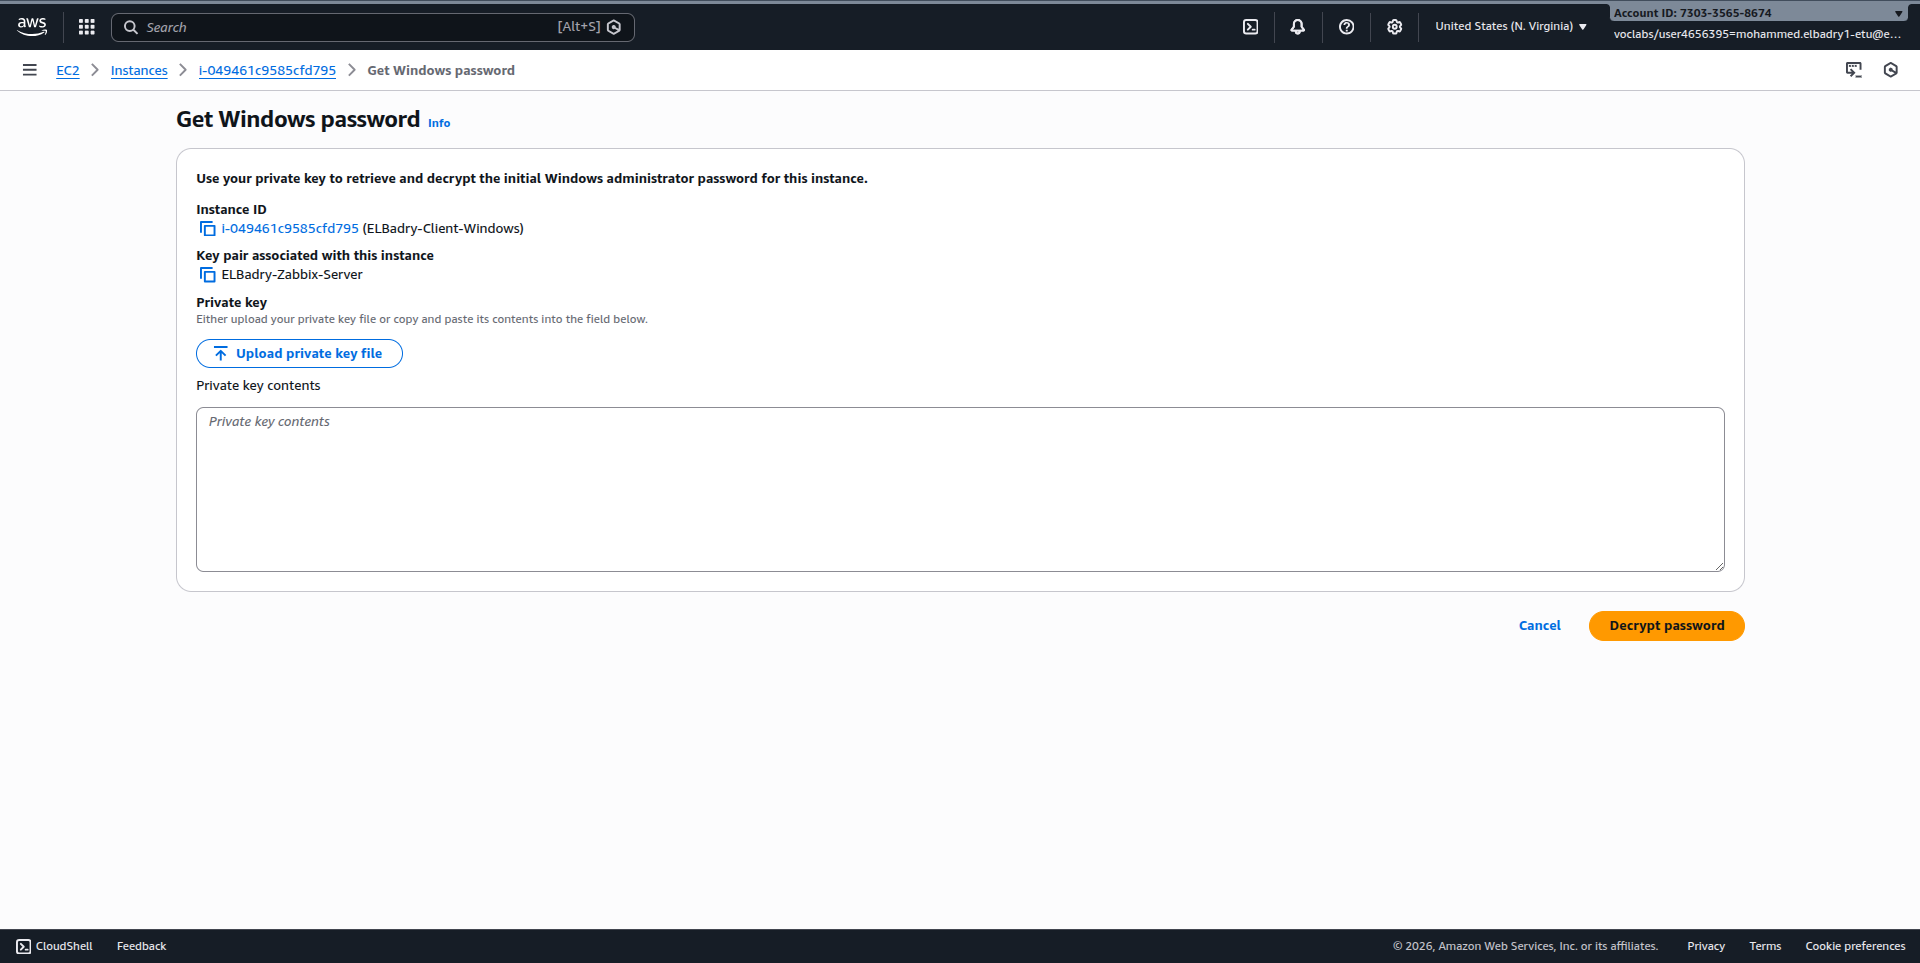
\includegraphics[width=0.85\textwidth]{images/12-windows-get-password.png}
\caption{Récupération du mot de passe Windows}
\label{fig:windows-password}
\end{figure}

\section{Connexion aux Instances}

\subsection{Connexion SSH au Serveur Zabbix}

\begin{lstlisting}[language=bash, caption=Connexion SSH au serveur Zabbix]
ssh -i "votre-cle.pem" ubuntu@<IP-PUBLIQUE-ZABBIX>
\end{lstlisting}

\begin{figure}[H]
\centering
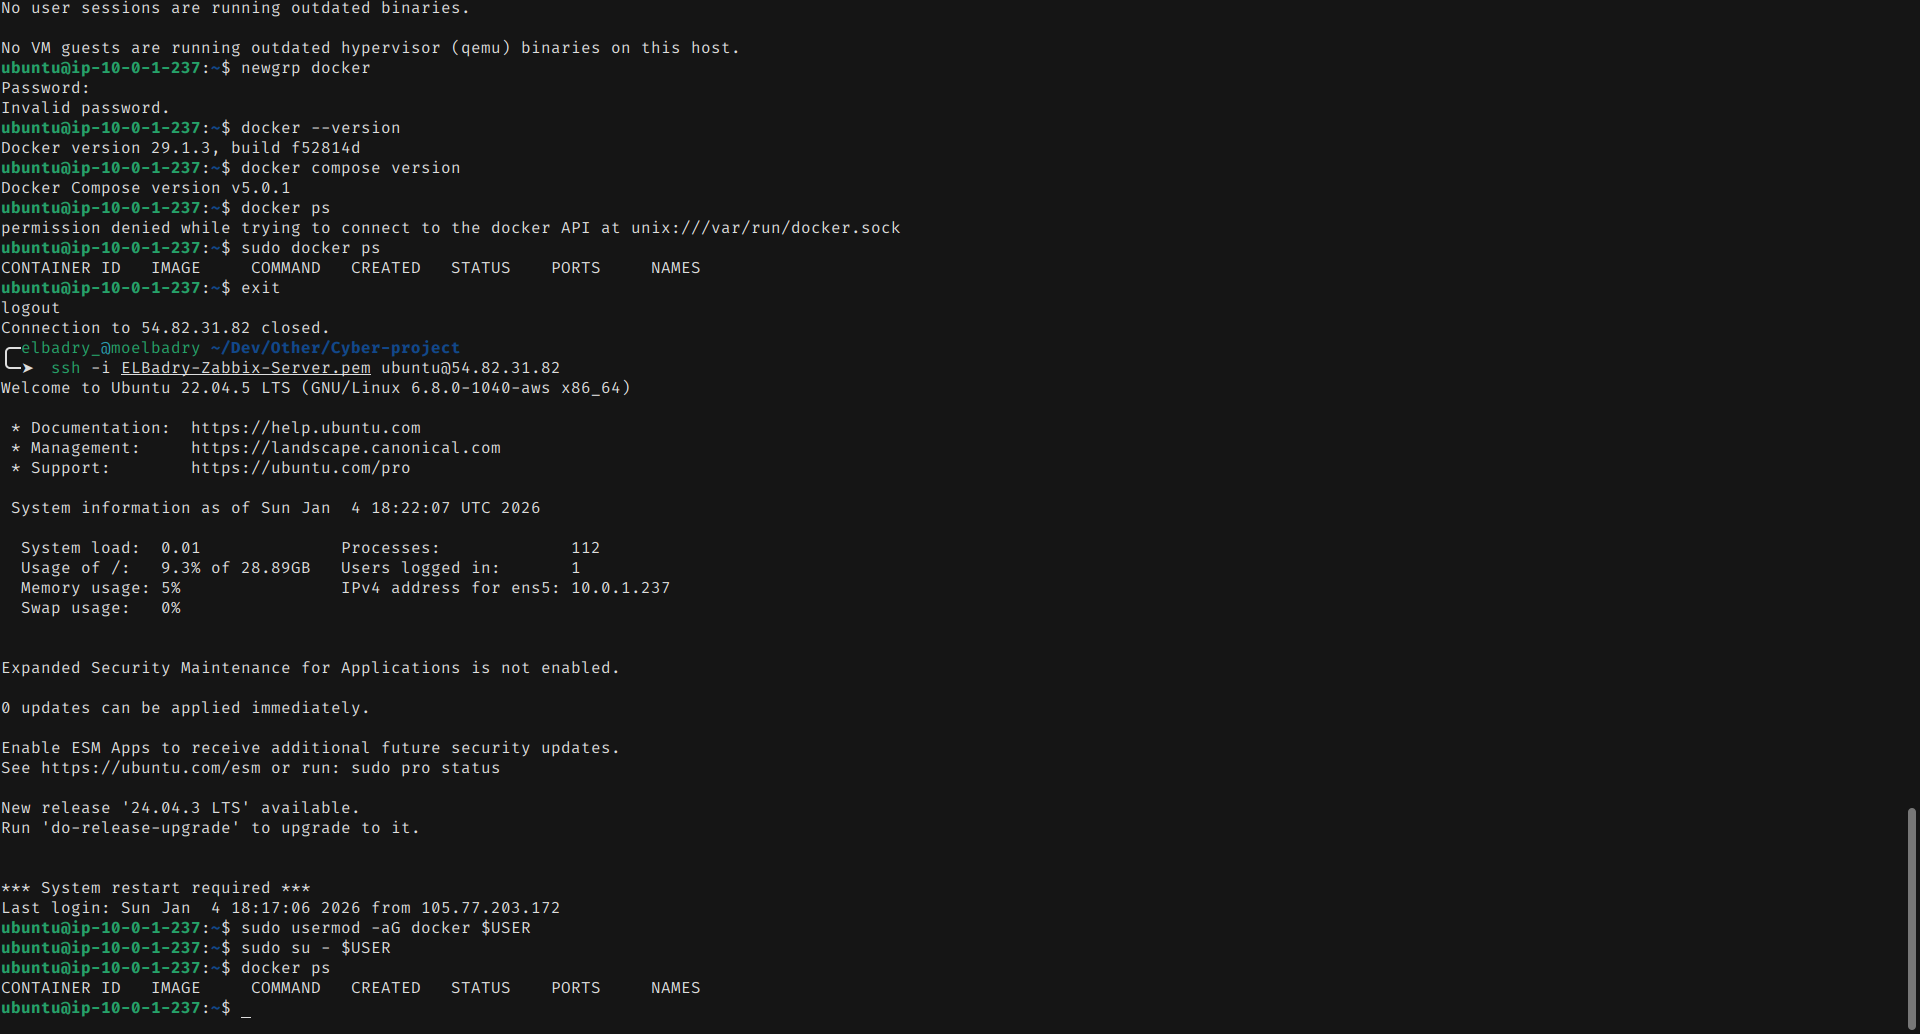
\includegraphics[width=0.95\textwidth]{images/13-ssh-connection-server.png}
\caption{Connexion SSH réussie au serveur Zabbix}
\label{fig:ssh-connection}
\end{figure}

\subsection{Connexion RDP au Client Windows}

\begin{enumerate}
    \item Ouvrir le client Bureau à distance (mstsc)
    \item Entrer l'IP publique de l'instance Windows
    \item Utiliser le nom d'utilisateur : \texttt{Administrator}
    \item Entrer le mot de passe déchiffré
\end{enumerate}

\begin{figure}[H]
\centering
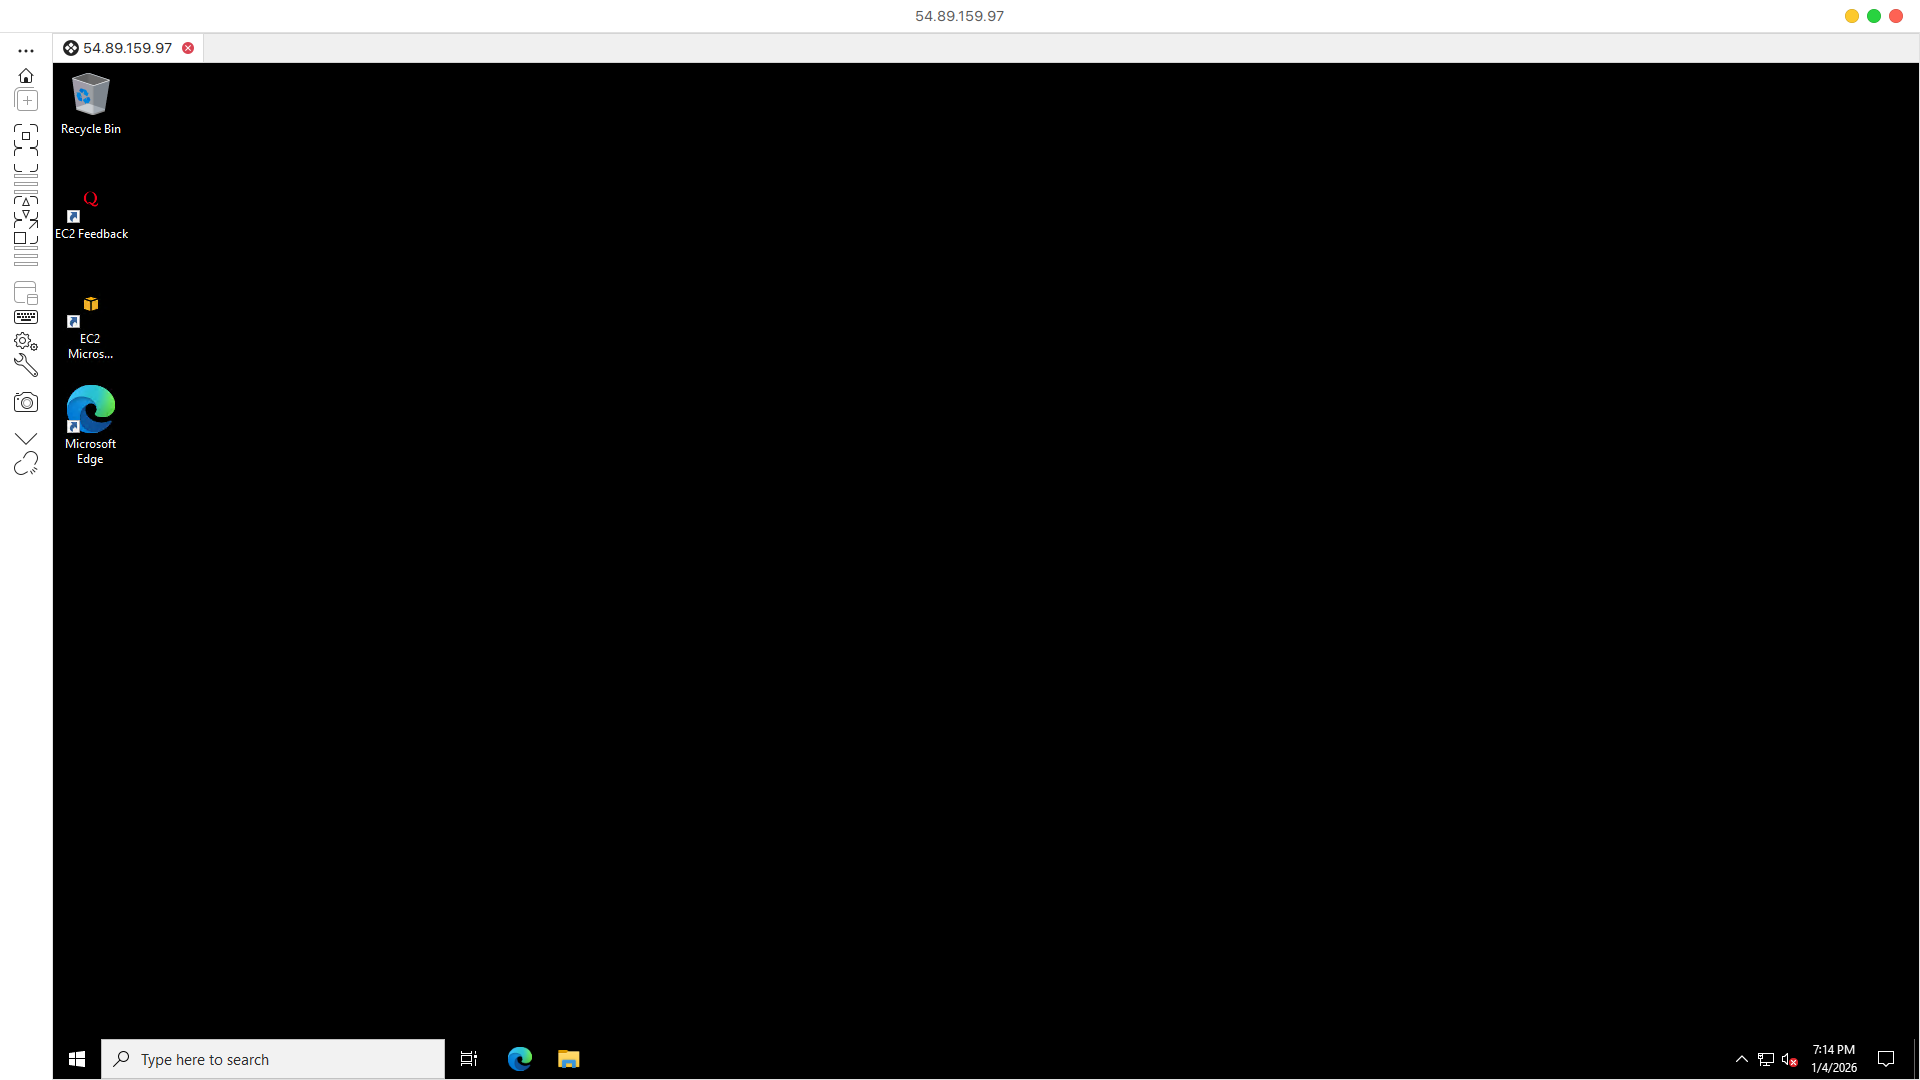
\includegraphics[width=0.85\textwidth]{images/21-windows-rdp-connection.png}
\caption{Connexion RDP au client Windows}
\label{fig:rdp-connection}
\end{figure}

\section{Tableau Récapitulatif}

\begin{table}[H]
\centering
\caption{Récapitulatif complet des instances}
\label{tab:instances-full}
\begin{tabular}{|l|c|c|c|}
\hline
\textbf{Propriété} & \textbf{Zabbix Server} & \textbf{Client Linux} & \textbf{Client Windows} \\
\hline
Type & t3.large & t3.medium & t3.large \\
\hline
vCPU & 2 & 2 & 2 \\
\hline
RAM & 8 Go & 4 Go & 8 Go \\
\hline
OS & Ubuntu 22.04 & Ubuntu 22.04 & Windows Server 2022 \\
\hline
Stockage & 30 Go & 20 Go & 30 Go \\
\hline
Accès & SSH (22) & SSH (22) & RDP (3389) \\
\hline
\end{tabular}
\end{table}

% ============================================
% Chapitre 4 : Déploiement Zabbix avec Docker
% ============================================
\chapter{Déploiement du Serveur Zabbix}
\label{chap:zabbix-deployment}

\section{Installation de Docker}

\subsection{Mise à jour du Système}

Après connexion au serveur Zabbix via SSH, la première étape consiste à mettre à jour le système :

\begin{lstlisting}[language=bash, caption=Mise à jour du système]
sudo apt update && sudo apt upgrade -y
\end{lstlisting}

\subsection{Installation de Docker Engine}

Installation de Docker et Docker Compose :

\begin{lstlisting}[language=bash, caption=Installation de Docker]
# Installation des prerequis
sudo apt install -y ca-certificates curl gnupg

# Ajout de la cle GPG Docker
sudo install -m 0755 -d /etc/apt/keyrings
curl -fsSL https://download.docker.com/linux/ubuntu/gpg | \
    sudo gpg --dearmor -o /etc/apt/keyrings/docker.gpg

# Ajout du repository Docker
echo "deb [arch=$(dpkg --print-architecture) \
    signed-by=/etc/apt/keyrings/docker.gpg] \
    https://download.docker.com/linux/ubuntu \
    $(lsb_release -cs) stable" | \
    sudo tee /etc/apt/sources.list.d/docker.list

# Installation de Docker
sudo apt update
sudo apt install -y docker-ce docker-ce-cli \
    containerd.io docker-compose-plugin

# Ajout de l'utilisateur au groupe docker
sudo usermod -aG docker $USER
\end{lstlisting}

\begin{figure}[H]
\centering
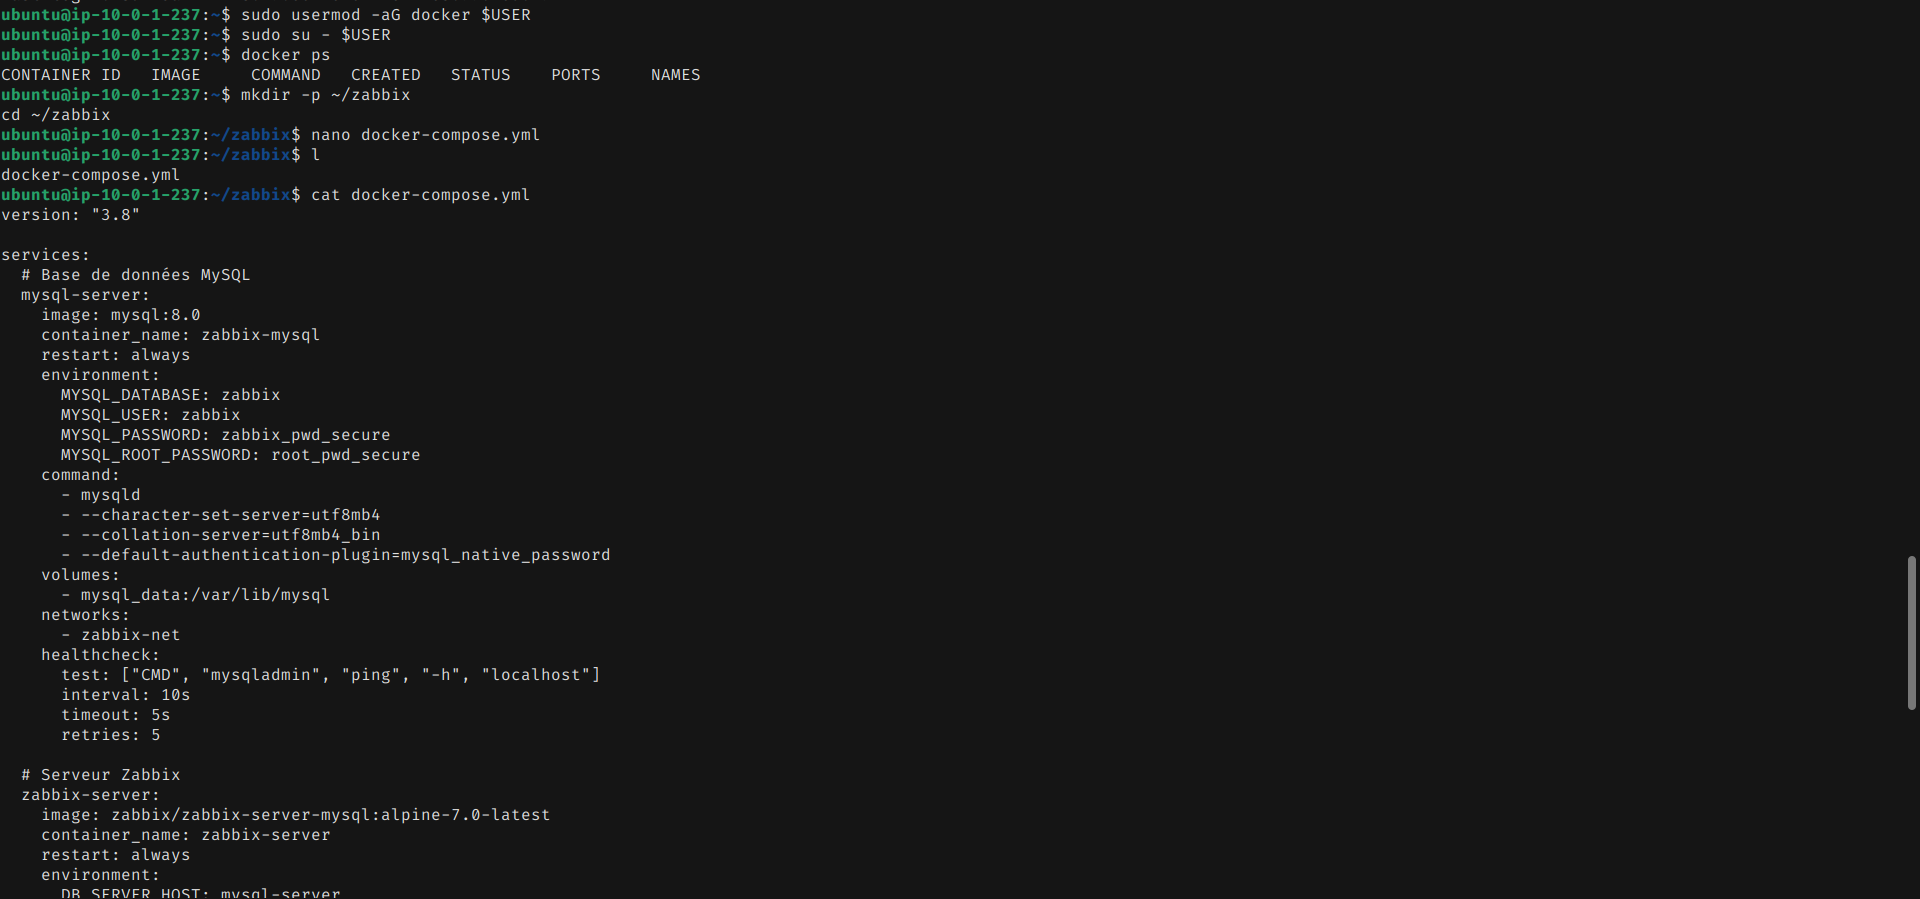
\includegraphics[width=0.95\textwidth]{images/15-docker-installation.png}
\caption{Installation de Docker réussie}
\label{fig:docker-installation}
\end{figure}

\subsection{Vérification de l'Installation}

\begin{lstlisting}[language=bash, caption=Vérification de Docker]
docker --version
docker compose version
\end{lstlisting}

\section{Configuration de Zabbix}

\subsection{Création du Fichier docker-compose.yml}

Le fichier docker-compose.yml définit l'ensemble de la stack Zabbix :

\begin{lstlisting}[language=bash, caption=Création du répertoire et du fichier]
mkdir ~/zabbix && cd ~/zabbix
nano docker-compose.yml
\end{lstlisting}

\begin{lstlisting}[caption=Contenu du docker-compose.yml, label=lst:docker-compose]
version: "3.8"

services:
  # Base de donnees MySQL
  mysql-server:
    image: mysql:8.0
    container_name: zabbix-mysql
    restart: always
    environment:
      MYSQL_DATABASE: zabbix
      MYSQL_USER: zabbix
      MYSQL_PASSWORD: zabbix_pwd_secure
      MYSQL_ROOT_PASSWORD: root_pwd_secure
    command:
      - mysqld
      - --character-set-server=utf8mb4
      - --collation-server=utf8mb4_bin
    volumes:
      - mysql_data:/var/lib/mysql
    networks:
      - zabbix-net

  # Serveur Zabbix
  zabbix-server:
    image: zabbix/zabbix-server-mysql:alpine-7.0-latest
    container_name: zabbix-server
    restart: always
    environment:
      DB_SERVER_HOST: mysql-server
      MYSQL_DATABASE: zabbix
      MYSQL_USER: zabbix
      MYSQL_PASSWORD: zabbix_pwd_secure
    ports:
      - "10051:10051"
    depends_on:
      - mysql-server
    networks:
      - zabbix-net

  # Interface Web Zabbix
  zabbix-web:
    image: zabbix/zabbix-web-nginx-mysql:alpine-7.0-latest
    container_name: zabbix-web
    restart: always
    environment:
      ZBX_SERVER_HOST: zabbix-server
      DB_SERVER_HOST: mysql-server
      MYSQL_DATABASE: zabbix
      MYSQL_USER: zabbix
      MYSQL_PASSWORD: zabbix_pwd_secure
      PHP_TZ: Europe/Paris
    ports:
      - "80:8080"
      - "443:8443"
    depends_on:
      - zabbix-server
    networks:
      - zabbix-net

  # Agent Zabbix local
  zabbix-agent:
    image: zabbix/zabbix-agent:alpine-7.0-latest
    container_name: zabbix-agent
    restart: always
    environment:
      ZBX_SERVER_HOST: zabbix-server
      ZBX_HOSTNAME: "Zabbix-Server"
    depends_on:
      - zabbix-server
    networks:
      - zabbix-net

volumes:
  mysql_data:

networks:
  zabbix-net:
    driver: bridge
\end{lstlisting}

\section{Lancement des Conteneurs}

\subsection{Démarrage de la Stack}

\begin{lstlisting}[language=bash, caption=Lancement de Zabbix]
docker compose up -d
\end{lstlisting}

\begin{figure}[H]
\centering
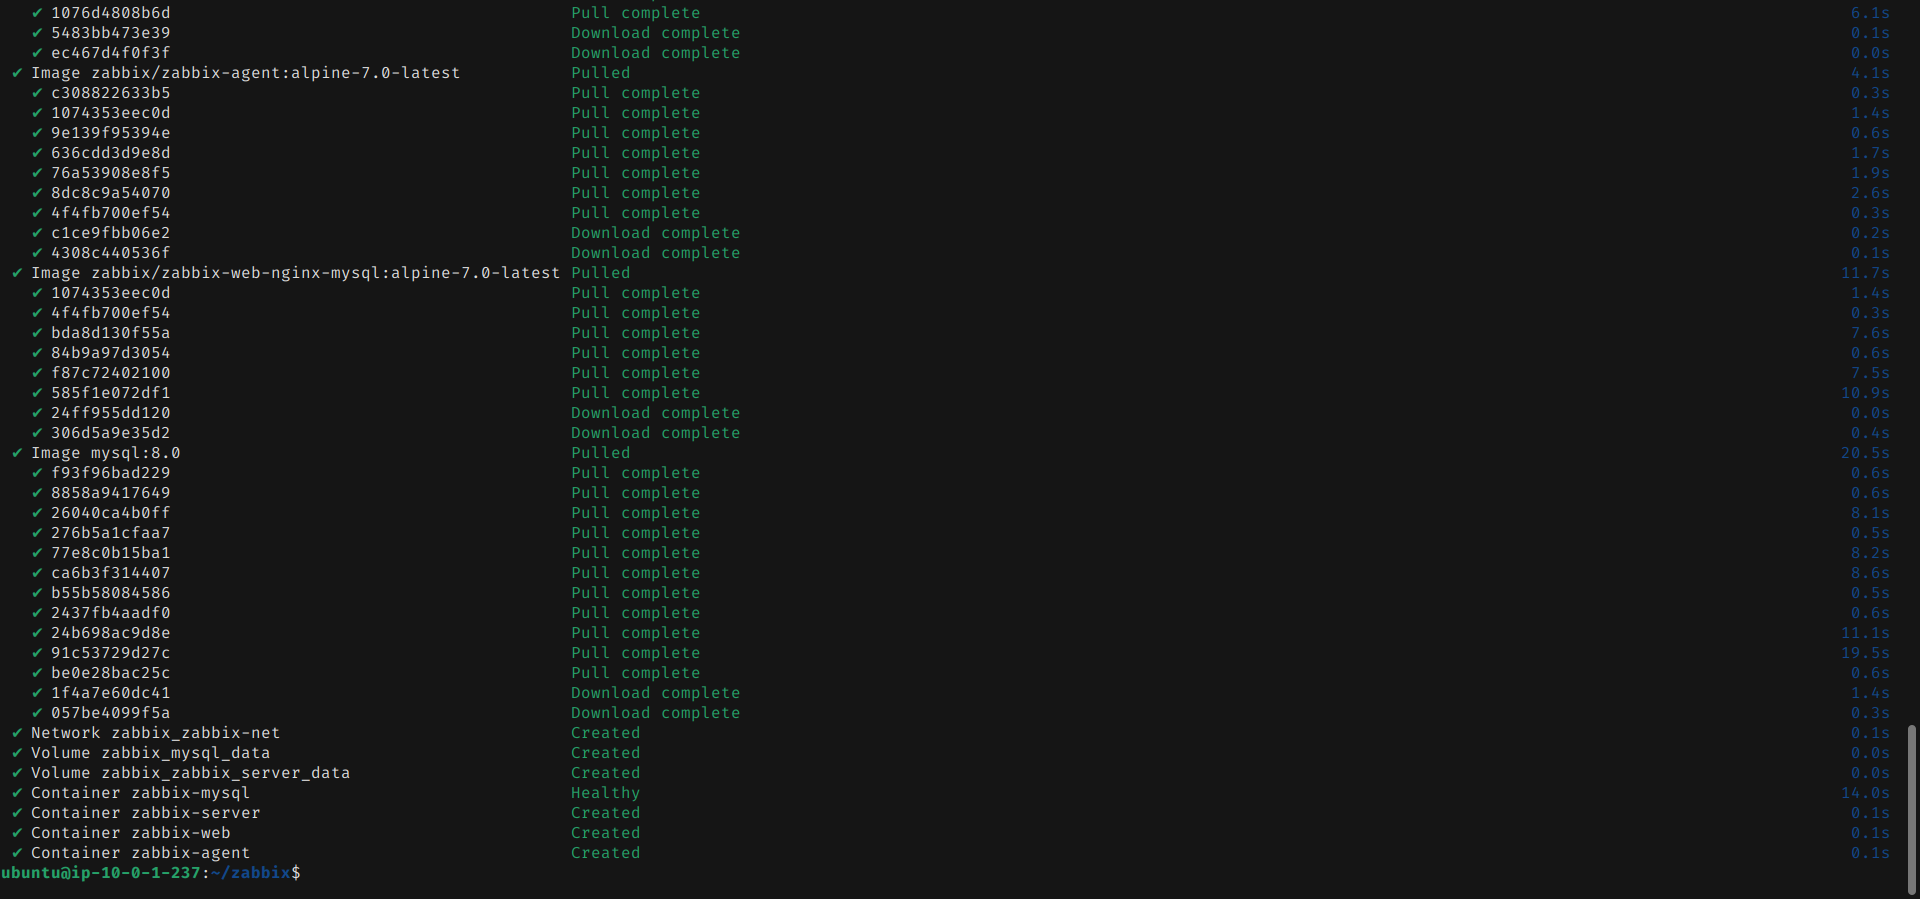
\includegraphics[width=0.95\textwidth]{images/16-docker-compose-up.png}
\caption{Lancement des conteneurs Docker}
\label{fig:docker-compose-up}
\end{figure}

\subsection{Vérification des Conteneurs}

\begin{lstlisting}[language=bash, caption=Vérification de l'état des conteneurs]
docker compose ps
\end{lstlisting}

\begin{figure}[H]
\centering
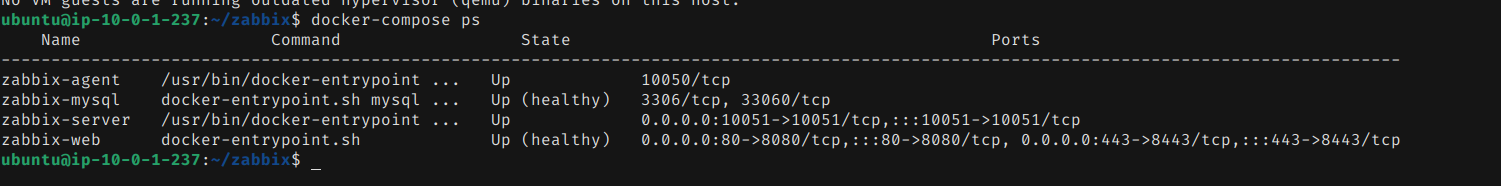
\includegraphics[width=0.95\textwidth]{images/17-containers-running-status.png}
\caption{Conteneurs Zabbix en cours d'exécution}
\label{fig:containers-running}
\end{figure}

Les 4 conteneurs doivent être en état \texttt{running} :
\begin{itemize}
    \item \textbf{zabbix-mysql} : Base de données MySQL 8.0
    \item \textbf{zabbix-server} : Serveur Zabbix 7.0
    \item \textbf{zabbix-web} : Interface Web Nginx
    \item \textbf{zabbix-agent} : Agent local
\end{itemize}

\section{Accès à l'Interface Web}

\subsection{Connexion à Zabbix}

L'interface Web est accessible via l'IP publique du serveur :

\begin{center}
\fbox{\parbox{0.6\textwidth}{
\centering
\textbf{URL :} \texttt{http://<IP-PUBLIQUE>}\\[0.2cm]
\textbf{Utilisateur :} Admin\\
\textbf{Mot de passe :} zabbix
}}
\end{center}

\begin{figure}[H]
\centering
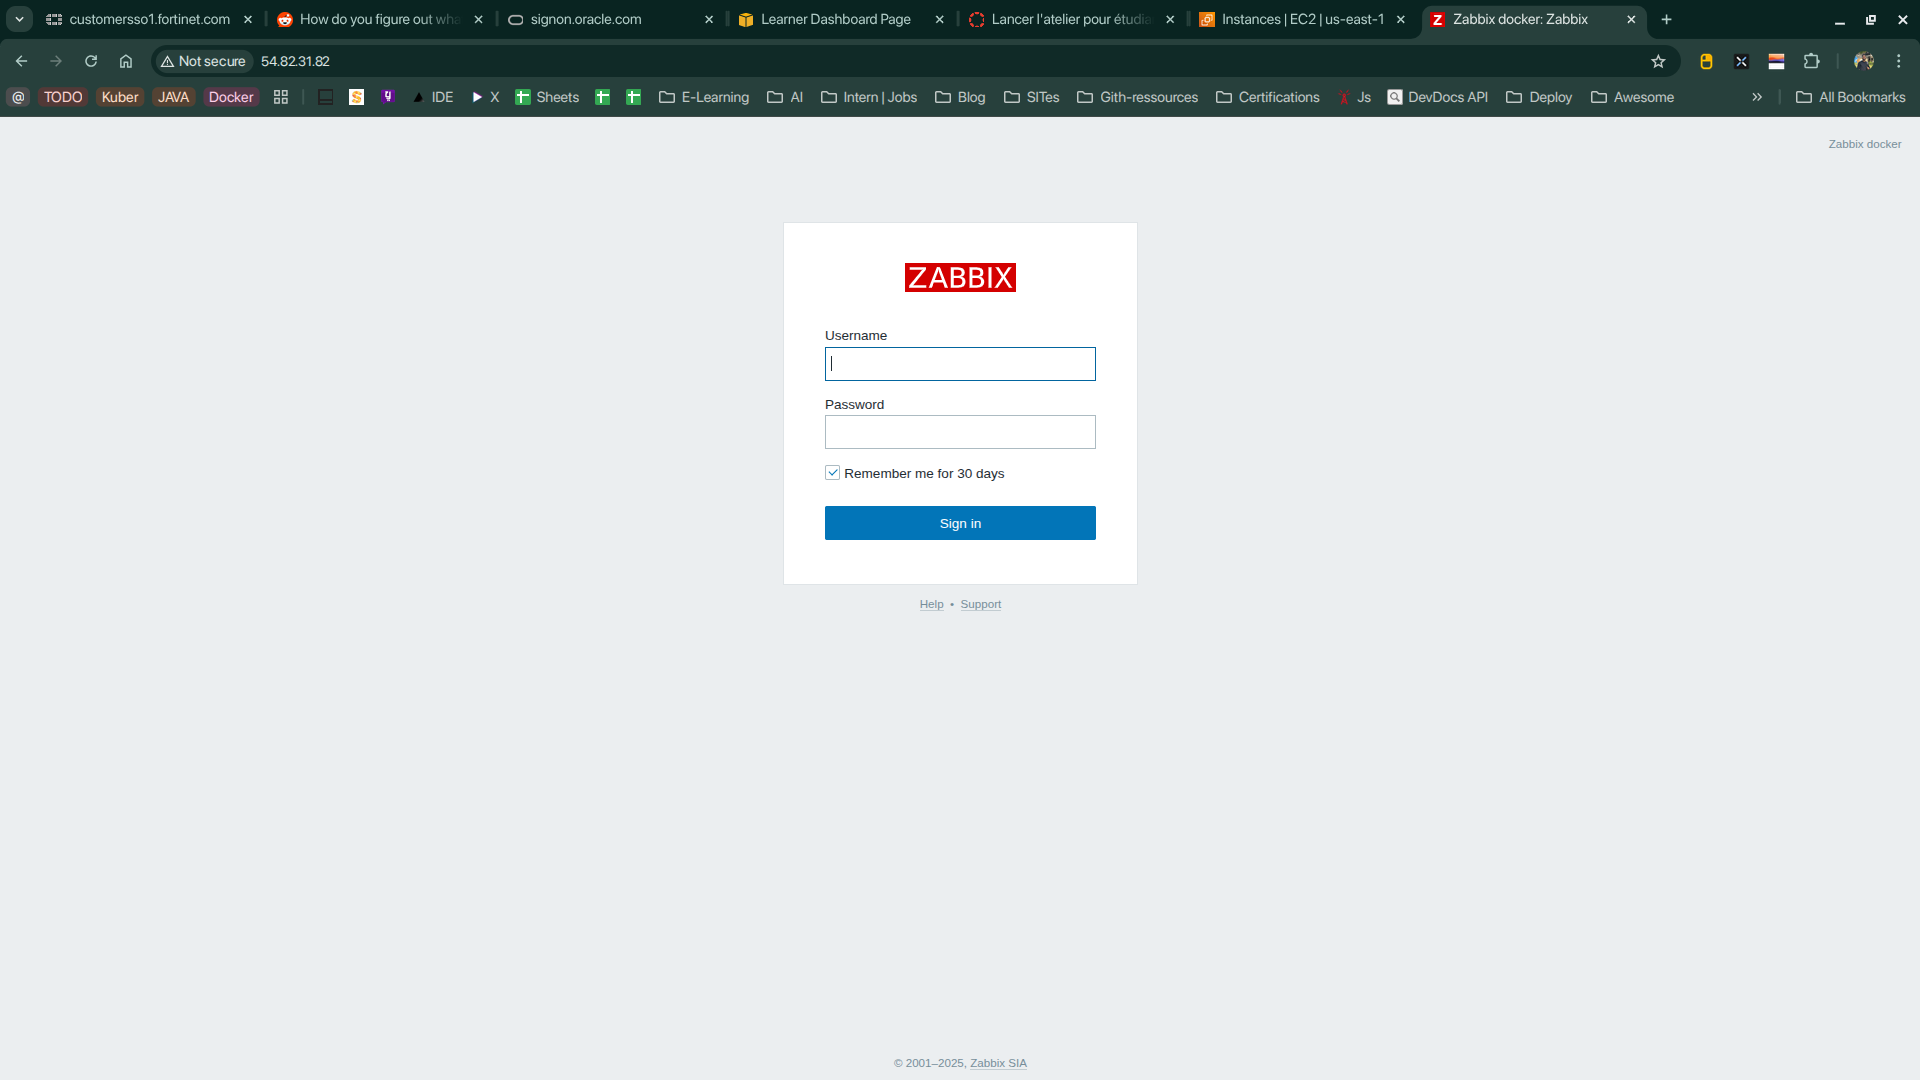
\includegraphics[width=0.85\textwidth]{images/18-zabbix-web-login.png}
\caption{Page de connexion Zabbix}
\label{fig:zabbix-login}
\end{figure}

\subsection{Dashboard Principal}

Après connexion, le tableau de bord principal de Zabbix s'affiche :

\begin{figure}[H]
\centering
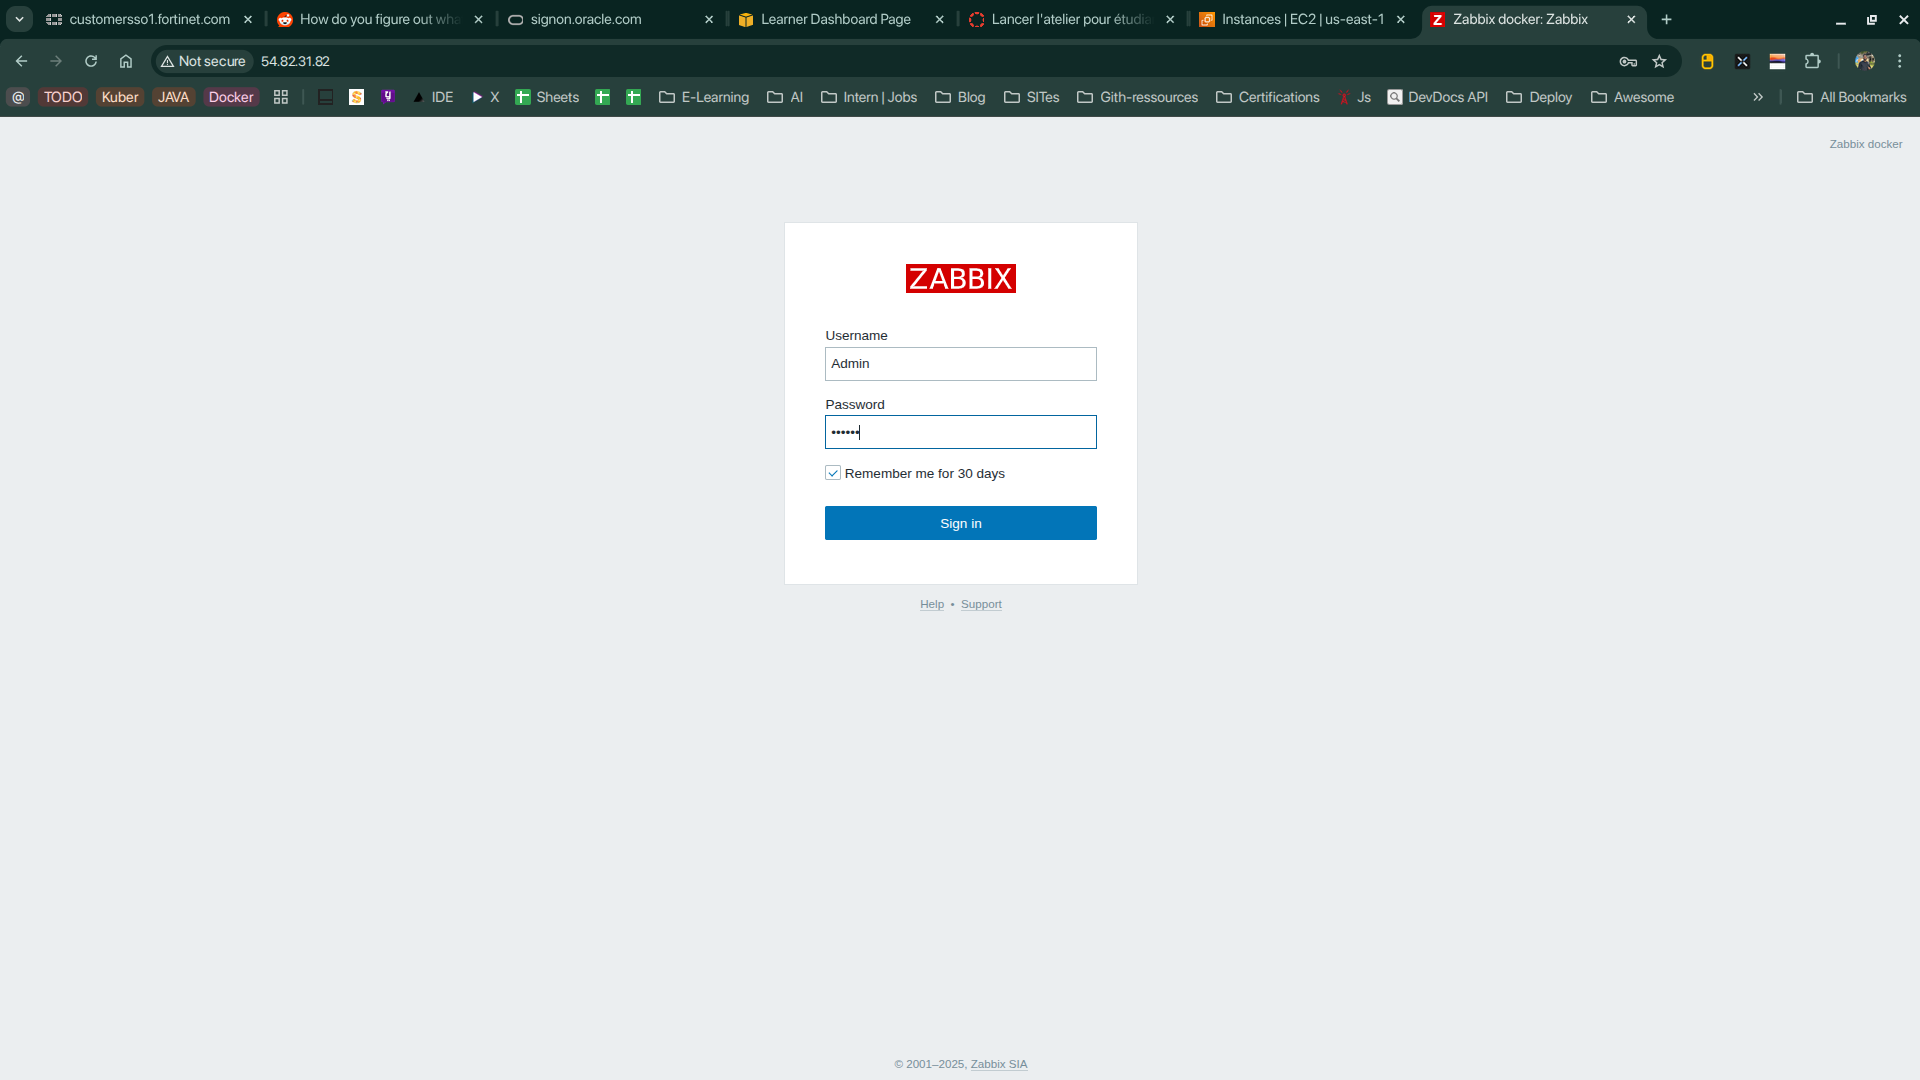
\includegraphics[width=0.95\textwidth]{images/19-zabbix-dashboard.png}
\caption{Dashboard principal de Zabbix}
\label{fig:zabbix-dashboard}
\end{figure}

\section{Architecture des Conteneurs}

\begin{figure}[H]
\centering
\begin{tikzpicture}[
    node distance=1cm,
    container/.style={rectangle, draw=bluecustom, line width=1.5pt, minimum width=3.5cm, minimum height=1cm, align=center, fill=bluecustom!10},
    arrow/.style={->, thick, >=stealth}
]

% Conteneurs
\node[container] (mysql) {MySQL 8.0\\Port 3306};
\node[container, right=2cm of mysql] (server) {Zabbix Server\\Port 10051};
\node[container, right=2cm of server] (web) {Zabbix Web\\Port 80/443};
\node[container, below=1.5cm of server] (agent) {Zabbix Agent\\Port 10050};

% Connexions
\draw[arrow] (server) -- (mysql) node[midway, above] {DB};
\draw[arrow] (web) -- (server) node[midway, above] {API};
\draw[arrow] (agent) -- (server) node[midway, right] {Metrics};

% Network
\node[draw=awsorange, dashed, line width=1pt, fit=(mysql)(server)(web)(agent), inner sep=0.5cm, label={[font=\small]below:zabbix-net (Docker Network)}] {};

\end{tikzpicture}
\caption{Architecture des conteneurs Docker}
\label{fig:docker-architecture}
\end{figure}

\section{Commandes Utiles}

\begin{table}[H]
\centering
\caption{Commandes Docker utiles}
\label{tab:docker-commands}
\begin{tabular}{|l|p{8cm}|}
\hline
\textbf{Commande} & \textbf{Description} \\
\hline
\texttt{docker compose up -d} & Démarrer les conteneurs \\
\hline
\texttt{docker compose down} & Arrêter les conteneurs \\
\hline
\texttt{docker compose ps} & Voir l'état des conteneurs \\
\hline
\texttt{docker compose logs -f} & Voir les logs en temps réel \\
\hline
\texttt{docker compose restart} & Redémarrer tous les conteneurs \\
\hline
\end{tabular}
\end{table}

% ============================================
% Chapitre 5 : Configuration des Agents
% ============================================
\chapter{Configuration des Clients (Agents)}
\label{chap:agents}

\section{Vue d'Ensemble}

Les agents Zabbix sont des logiciels installés sur les machines à superviser. Ils collectent les métriques système et les transmettent au serveur Zabbix.

\begin{table}[H]
\centering
\caption{Modes de communication des agents}
\label{tab:agent-modes}
\begin{tabular}{|l|p{10cm}|}
\hline
\textbf{Mode} & \textbf{Description} \\
\hline
Passif & Le serveur interroge l'agent (port 10050) \\
\hline
Actif & L'agent envoie les données au serveur (port 10051) \\
\hline
\end{tabular}
\end{table}

\section{Installation sur Linux (Ubuntu)}

\subsection{Connexion au Client Linux}

\begin{lstlisting}[language=bash, caption=Connexion SSH au client Linux]
ssh -i "votre-cle.pem" ubuntu@<IP-CLIENT-LINUX>
\end{lstlisting}

\subsection{Installation de l'Agent Zabbix}

\begin{lstlisting}[language=bash, caption=Installation de l'agent Zabbix sur Ubuntu]
# Telecharger le package Zabbix
wget https://repo.zabbix.com/zabbix/7.0/ubuntu/pool/main/z/\
zabbix-release/zabbix-release_latest_7.0+ubuntu22.04_all.deb

# Installer le package
sudo dpkg -i zabbix-release_latest_7.0+ubuntu22.04_all.deb

# Mettre a jour et installer l'agent
sudo apt update
sudo apt install -y zabbix-agent
\end{lstlisting}

\subsection{Configuration de l'Agent Linux}

Éditer le fichier de configuration :

\begin{lstlisting}[language=bash, caption=Édition de la configuration]
sudo nano /etc/zabbix/zabbix_agentd.conf
\end{lstlisting}

Modifier les paramètres suivants :

\begin{lstlisting}[caption=Configuration zabbix\_agentd.conf (Linux)]
# Adresse IP du serveur Zabbix (IP privee)
Server=10.0.1.X

# Pour le mode actif
ServerActive=10.0.1.X

# Nom d'hote (doit correspondre dans Zabbix)
Hostname=ELBadry-Client-Linux

# Autoriser les commandes a distance (optionnel)
EnableRemoteCommands=1
\end{lstlisting}

\begin{figure}[H]
\centering
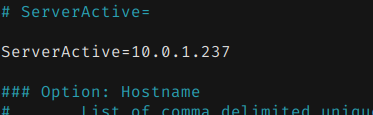
\includegraphics[width=0.95\textwidth]{images/20-agent-linux-configuration.png}
\caption{Configuration de l'agent Zabbix sur Linux}
\label{fig:agent-linux-config}
\end{figure}

\subsection{Démarrage du Service}

\begin{lstlisting}[language=bash, caption=Démarrage de l'agent Linux]
# Redemarrer l'agent
sudo systemctl restart zabbix-agent

# Activer au demarrage
sudo systemctl enable zabbix-agent

# Verifier le statut
sudo systemctl status zabbix-agent
\end{lstlisting}

\subsection{Vérification de la Connectivité}

\begin{lstlisting}[language=bash, caption=Test de connectivité]
# Verifier que l'agent ecoute sur le port 10050
sudo netstat -tlnp | grep 10050

# Tester la connexion depuis le serveur Zabbix
zabbix_get -s <IP-CLIENT-LINUX> -k agent.ping
\end{lstlisting}

\section{Installation sur Windows}

\subsection{Connexion RDP}

Se connecter au client Windows via Remote Desktop :
\begin{enumerate}
    \item Ouvrir \texttt{mstsc.exe}
    \item Entrer l'IP publique du client Windows
    \item Utiliser les credentials récupérés (Administrator)
\end{enumerate}

\begin{figure}[H]
\centering
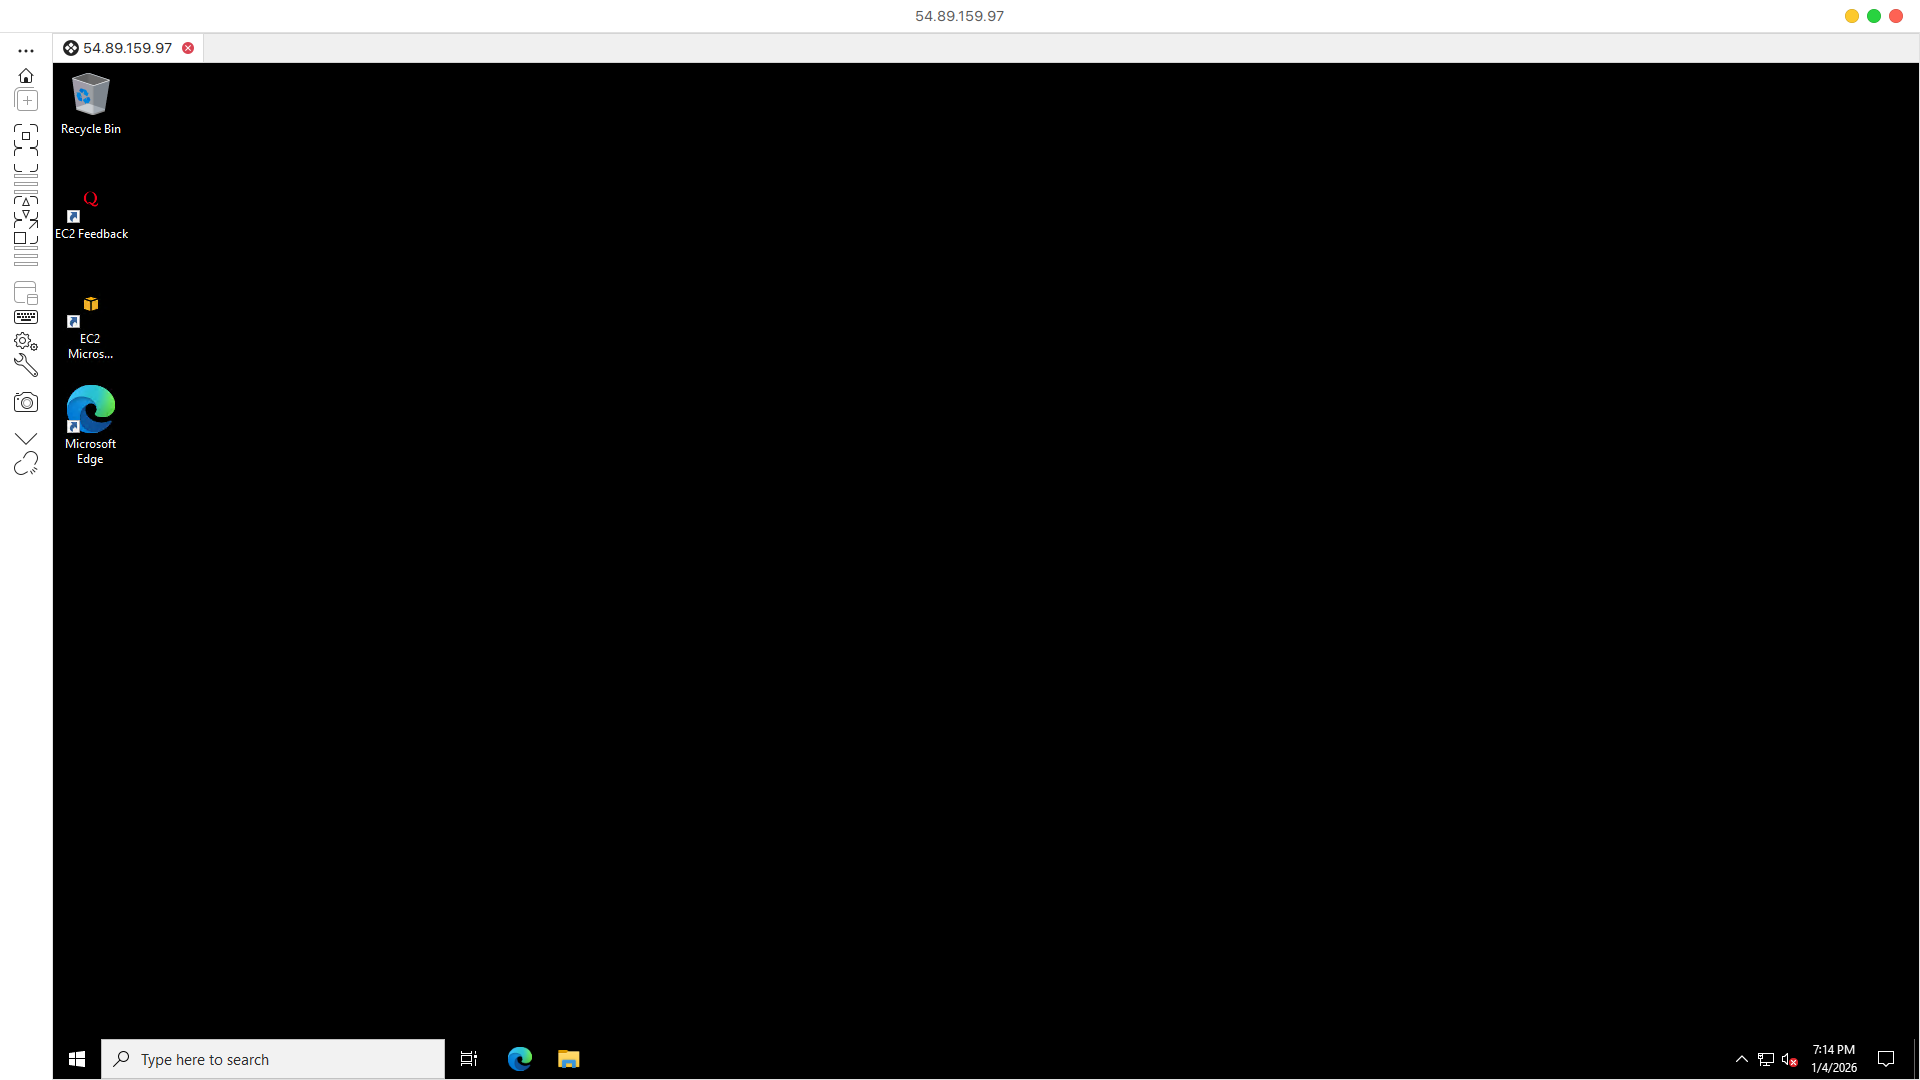
\includegraphics[width=0.85\textwidth]{images/21-windows-rdp-connection.png}
\caption{Connexion RDP au client Windows}
\label{fig:windows-rdp}
\end{figure}

\subsection{Téléchargement de l'Agent}

\begin{enumerate}
    \item Ouvrir le navigateur sur le serveur Windows
    \item Aller sur : \url{https://www.zabbix.com/download_agents}
    \item Sélectionner :
    \begin{itemize}
        \item OS : Windows
        \item Version : 7.0 LTS
        \item Architecture : AMD64
        \item Format : MSI
    \end{itemize}
    \item Télécharger le fichier MSI
\end{enumerate}

\subsection{Installation de l'Agent Windows}

\begin{enumerate}
    \item Exécuter le fichier MSI téléchargé
    \item Configurer les paramètres :
    \begin{itemize}
        \item \textbf{Zabbix Server IP} : IP privée du serveur (10.0.1.X)
        \item \textbf{Agent Hostname} : ELBadry-Client-Windows
        \item \textbf{Listen Port} : 10050
    \end{itemize}
    \item Terminer l'installation
\end{enumerate}

\begin{figure}[H]
\centering
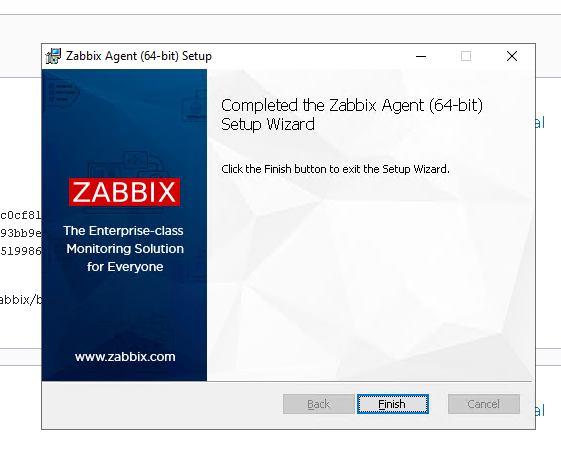
\includegraphics[width=0.85\textwidth]{images/22-agent-windows-installation.png}
\caption{Installation de l'agent Zabbix sur Windows}
\label{fig:agent-windows-install}
\end{figure}

\subsection{Vérification du Service Windows}

\begin{enumerate}
    \item Ouvrir \texttt{services.msc}
    \item Rechercher "Zabbix Agent"
    \item Vérifier que le service est en état "Running"
\end{enumerate}

\subsection{Configuration du Pare-feu Windows}

S'assurer que le port 10050 est ouvert :

\begin{enumerate}
    \item Ouvrir Windows Firewall
    \item Créer une règle entrante pour le port TCP 10050
    \item Autoriser les connexions
\end{enumerate}

\section{Ajout des Hôtes dans Zabbix}

\subsection{Ajouter le Client Linux}

\begin{enumerate}
    \item Dans Zabbix Web : \textbf{Data collection → Hosts → Create host}
    \item Configurer :
    \begin{itemize}
        \item \textbf{Host name} : ELBadry-Client-Linux
        \item \textbf{Groups} : Linux servers
        \item \textbf{Interfaces} : Agent, IP = 10.0.1.X, Port = 10050
    \end{itemize}
    \item Dans l'onglet \textbf{Templates} : Ajouter "Linux by Zabbix agent"
    \item Cliquer sur \textbf{Add}
\end{enumerate}

\begin{figure}[H]
\centering
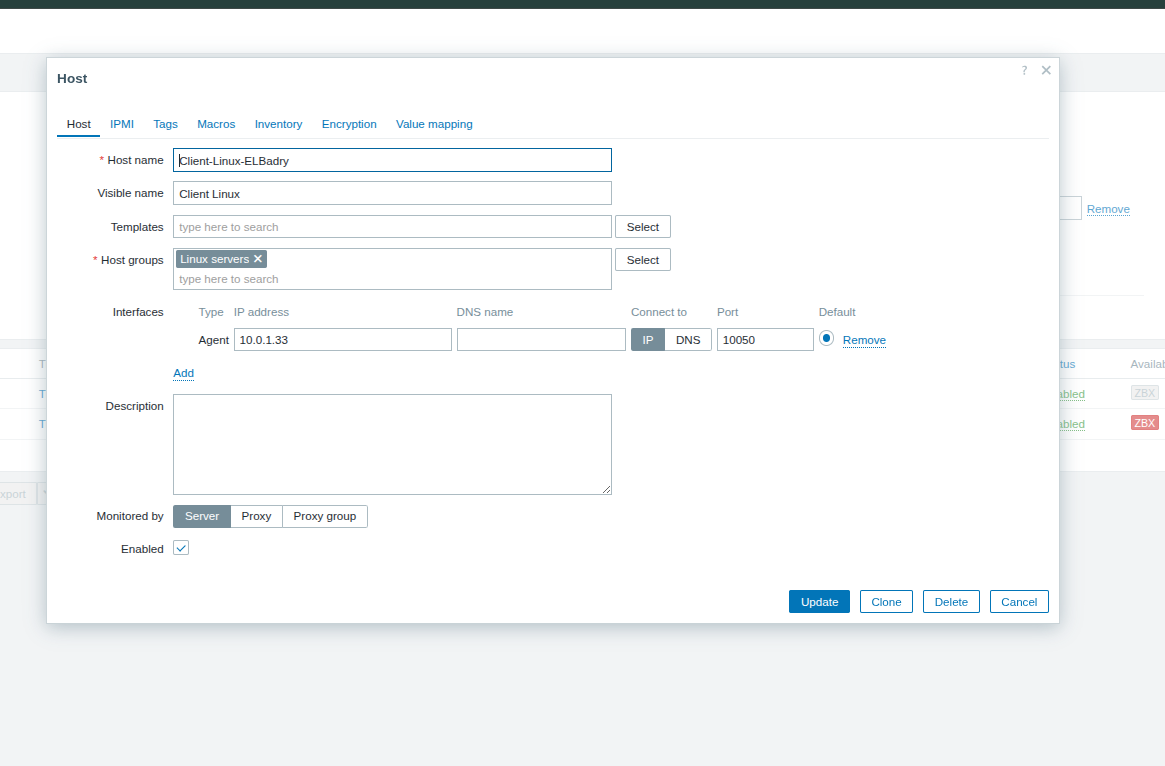
\includegraphics[width=0.95\textwidth]{images/23-zabbix-add-host-linux.png}
\caption{Ajout du client Linux dans Zabbix}
\label{fig:add-host-linux}
\end{figure}

\subsection{Ajouter le Client Windows}

\begin{enumerate}
    \item \textbf{Data collection → Hosts → Create host}
    \item Configurer :
    \begin{itemize}
        \item \textbf{Host name} : ELBadry-Client-Windows
        \item \textbf{Groups} : Windows servers (créer si nécessaire)
        \item \textbf{Interfaces} : Agent, IP = 10.0.1.X, Port = 10050
    \end{itemize}
    \item Dans l'onglet \textbf{Templates} : Ajouter "Windows by Zabbix agent"
    \item Cliquer sur \textbf{Add}
\end{enumerate}

\section{Vérification de la Connexion}

\subsection{Liste des Hôtes}

\begin{figure}[H]
\centering
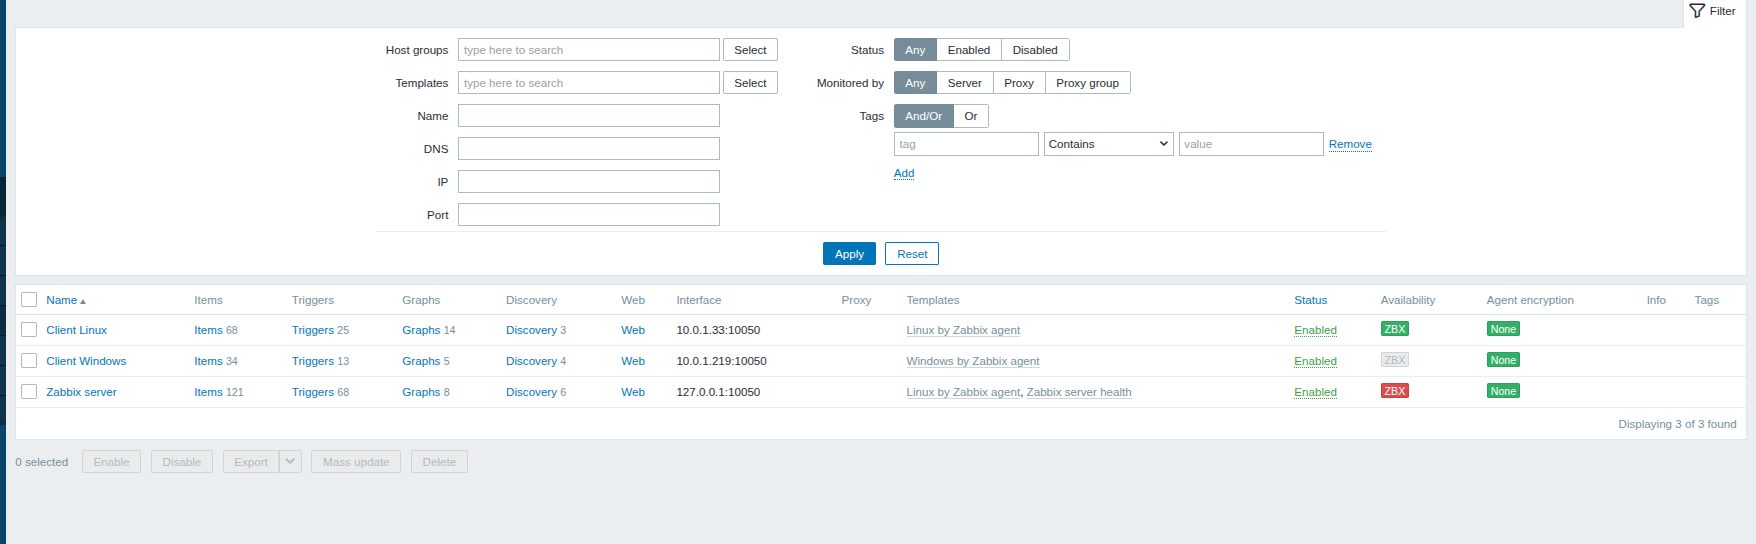
\includegraphics[width=0.95\textwidth]{images/24-zabbix-hosts-list.png}
\caption{Liste des hôtes configurés dans Zabbix}
\label{fig:hosts-list}
\end{figure}

\subsection{Statut des Agents (ZBX Vert)}

Le statut "ZBX" vert indique que l'agent est correctement connecté et répond aux requêtes du serveur.

\begin{figure}[H]
\centering
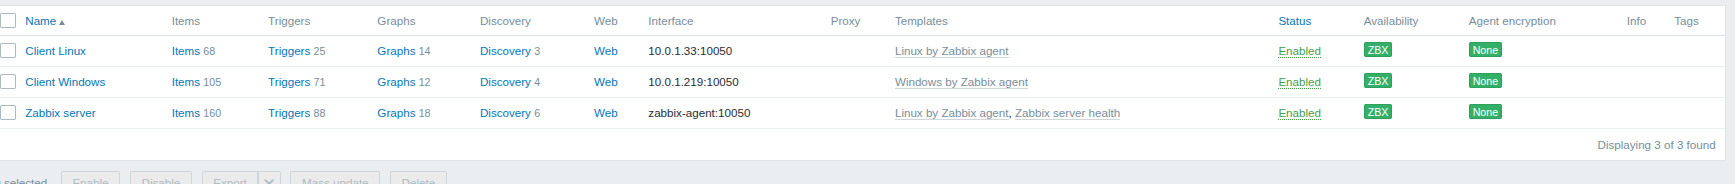
\includegraphics[width=0.95\textwidth]{images/25-zabbix-hosts-status-green.png}
\caption{Statut ZBX vert - Agents connectés avec succès}
\label{fig:zbx-green}
\end{figure}

\section{Tableau Récapitulatif des Agents}

\begin{table}[H]
\centering
\caption{Configuration des agents}
\label{tab:agents-config}
\begin{tabular}{|l|c|c|}
\hline
\textbf{Propriété} & \textbf{Client Linux} & \textbf{Client Windows} \\
\hline
Hostname & ELBadry-Client-Linux & ELBadry-Client-Windows \\
\hline
IP Privée & 10.0.1.X & 10.0.1.X \\
\hline
Port & 10050 & 10050 \\
\hline
Template & Linux by Zabbix agent & Windows by Zabbix agent \\
\hline
Version Agent & 7.0 & 7.0 \\
\hline
\end{tabular}
\end{table}

% ============================================
% Chapitre 6 : Monitoring et Tableaux de Bord
% ============================================
\chapter{Monitoring et Tableaux de Bord}
\label{chap:monitoring}

\section{Vue d'Ensemble du Monitoring}

Une fois les agents configurés et connectés, Zabbix collecte automatiquement les métriques des hôtes supervisés. Cette section présente les fonctionnalités de monitoring et de visualisation.

\section{Dashboard Principal}

Le tableau de bord principal de Zabbix affiche une vue synthétique de l'état de l'infrastructure :

\begin{figure}[H]
\centering
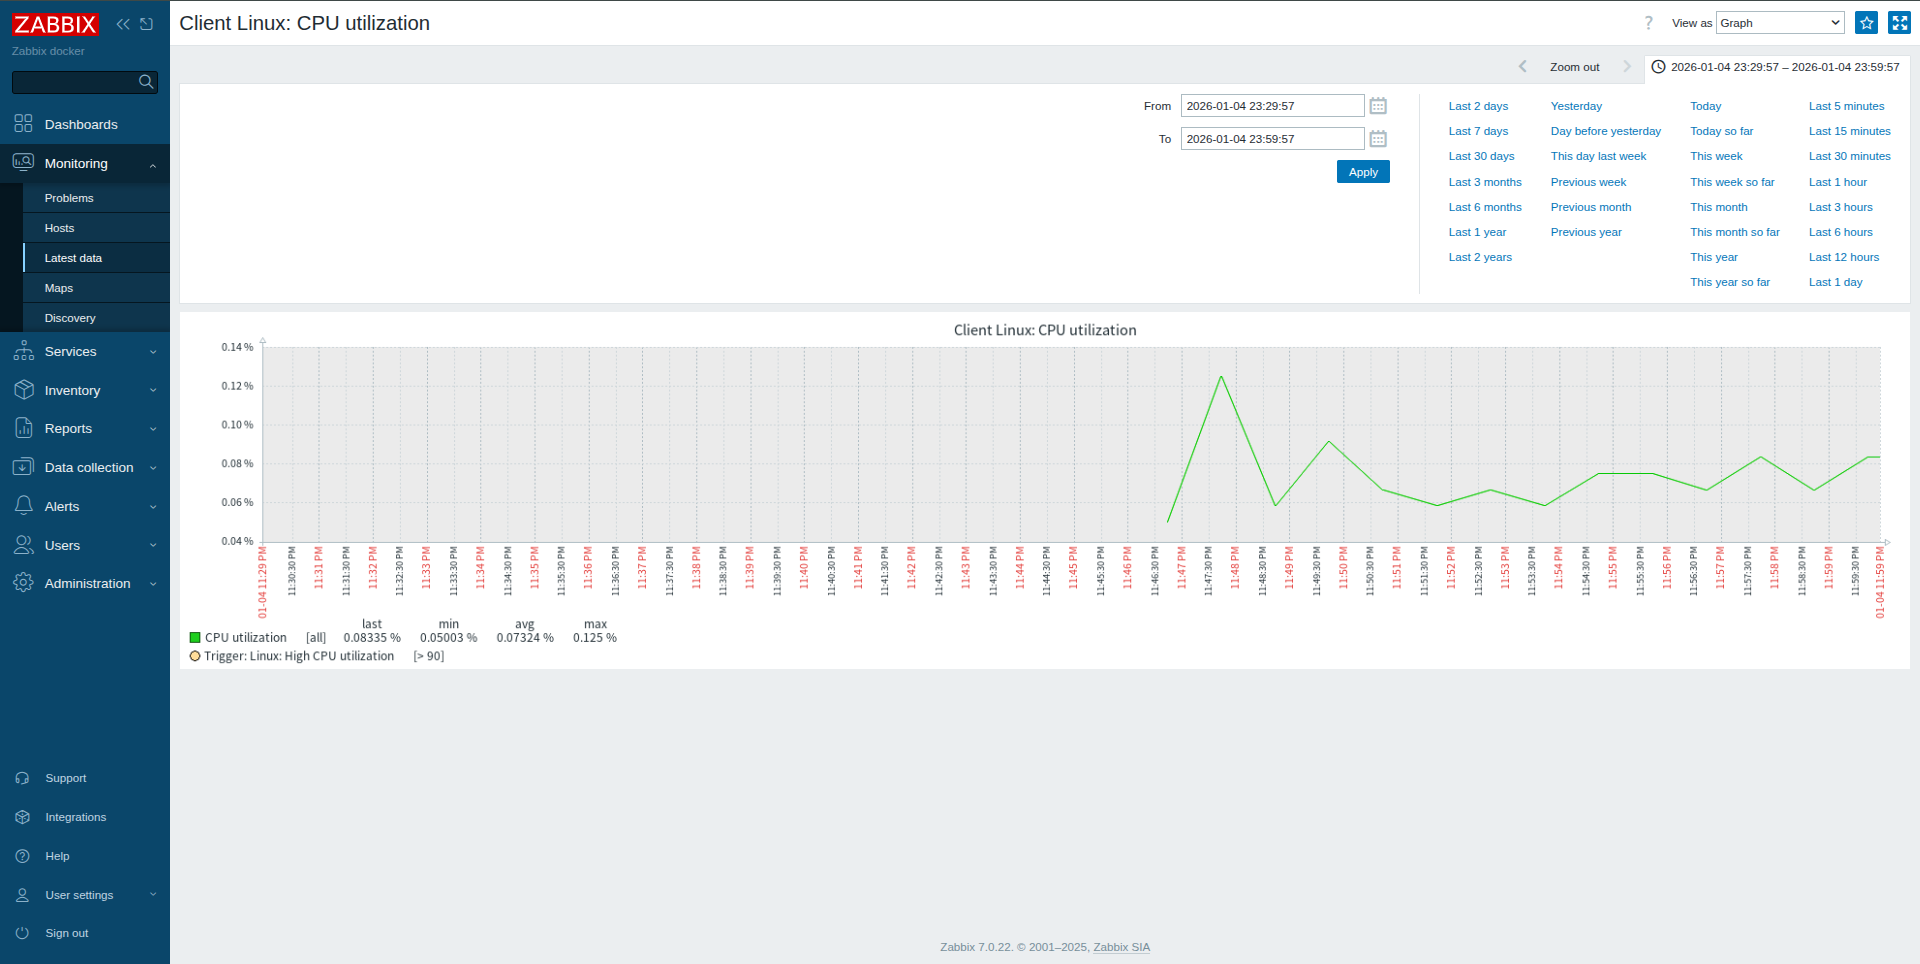
\includegraphics[width=0.95\textwidth]{images/26-zabbix-monitoring-dashboard.png}
\caption{Dashboard de monitoring Zabbix}
\label{fig:monitoring-dashboard}
\end{figure}

\section{Métriques Collectées}

\subsection{Métriques Système Linux}

Le template "Linux by Zabbix agent" collecte automatiquement :

\begin{table}[H]
\centering
\caption{Métriques Linux collectées}
\label{tab:linux-metrics}
\begin{tabular}{|l|p{8cm}|}
\hline
\textbf{Catégorie} & \textbf{Métriques} \\
\hline
CPU & Utilisation, load average, temps utilisateur/système \\
\hline
Mémoire & RAM utilisée/libre, swap, cache \\
\hline
Disque & Espace utilisé, I/O, inodes \\
\hline
Réseau & Trafic entrant/sortant, erreurs, paquets \\
\hline
Processus & Nombre de processus, zombies \\
\hline
Système & Uptime, hostname, version OS \\
\hline
\end{tabular}
\end{table}

\subsection{Métriques Système Windows}

Le template "Windows by Zabbix agent" collecte :

\begin{table}[H]
\centering
\caption{Métriques Windows collectées}
\label{tab:windows-metrics}
\begin{tabular}{|l|p{8cm}|}
\hline
\textbf{Catégorie} & \textbf{Métriques} \\
\hline
CPU & Utilisation par cœur, temps processeur \\
\hline
Mémoire & Mémoire physique, mémoire virtuelle, page file \\
\hline
Disque & Espace disque, temps de lecture/écriture \\
\hline
Réseau & Bande passante, erreurs d'interface \\
\hline
Services & État des services Windows \\
\hline
Événements & Logs Windows (Système, Application) \\
\hline
\end{tabular}
\end{table}

\section{Test de Charge (Stress Test)}

\subsection{Objectif}

Pour démontrer la capacité de Zabbix à détecter les anomalies, nous effectuons un test de charge CPU sur le client Linux.

\subsection{Exécution du Test}

\begin{lstlisting}[language=bash, caption=Installation et exécution de stress]
# Installation de l'outil stress
sudo apt install -y stress

# Lancement du stress test CPU (4 coeurs pendant 60s)
stress --cpu 4 --timeout 60s
\end{lstlisting}

\begin{figure}[H]
\centering
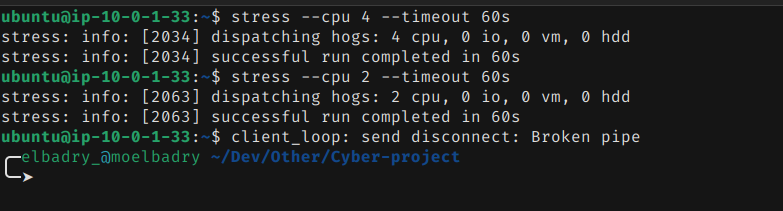
\includegraphics[width=0.95\textwidth]{images/27-stress-test-command.png}
\caption{Exécution de la commande stress}
\label{fig:stress-command}
\end{figure}

\subsection{Observation dans Zabbix}

Le pic de CPU est immédiatement visible dans les graphiques Zabbix :

\begin{figure}[H]
\centering
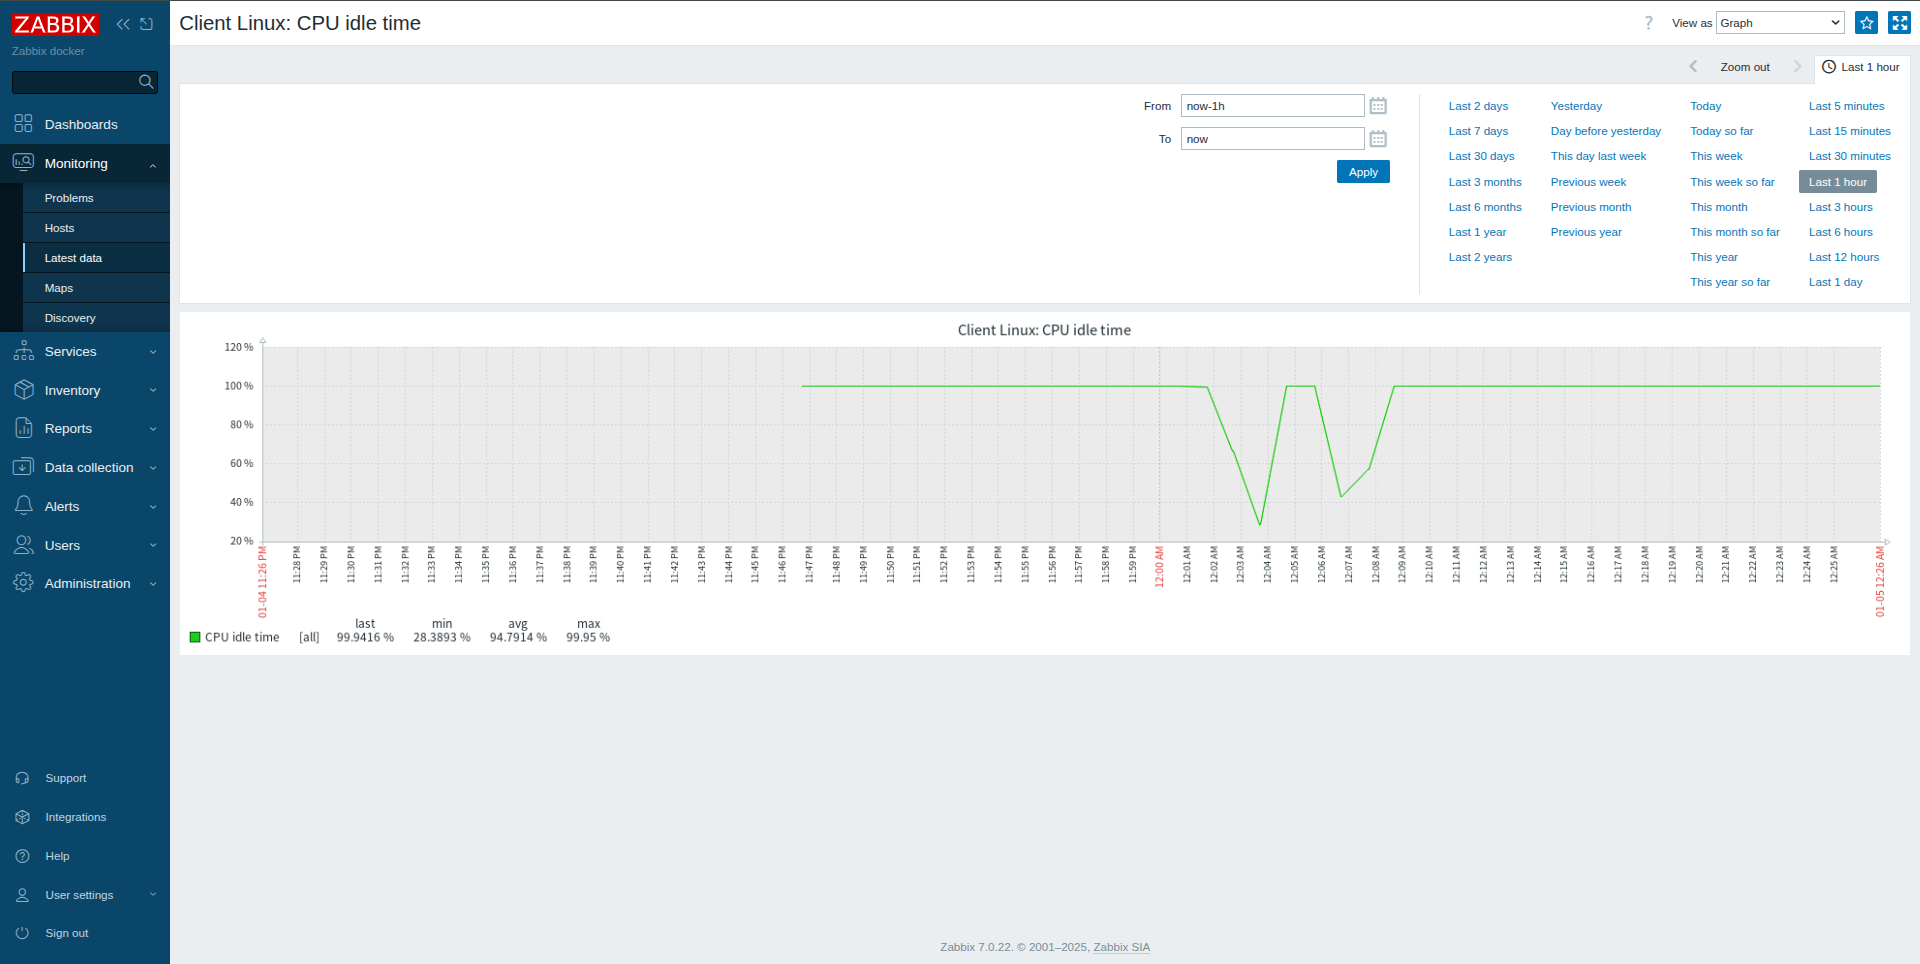
\includegraphics[width=0.95\textwidth]{images/28-stress-test-cpu-spike.png}
\caption{Pic de CPU détecté suite au stress test}
\label{fig:cpu-spike}
\end{figure}

\section{Gestion des Alertes}

\subsection{Problèmes Détectés}

Zabbix déclenche automatiquement des alertes basées sur les triggers prédéfinis :

\begin{figure}[H]
\centering
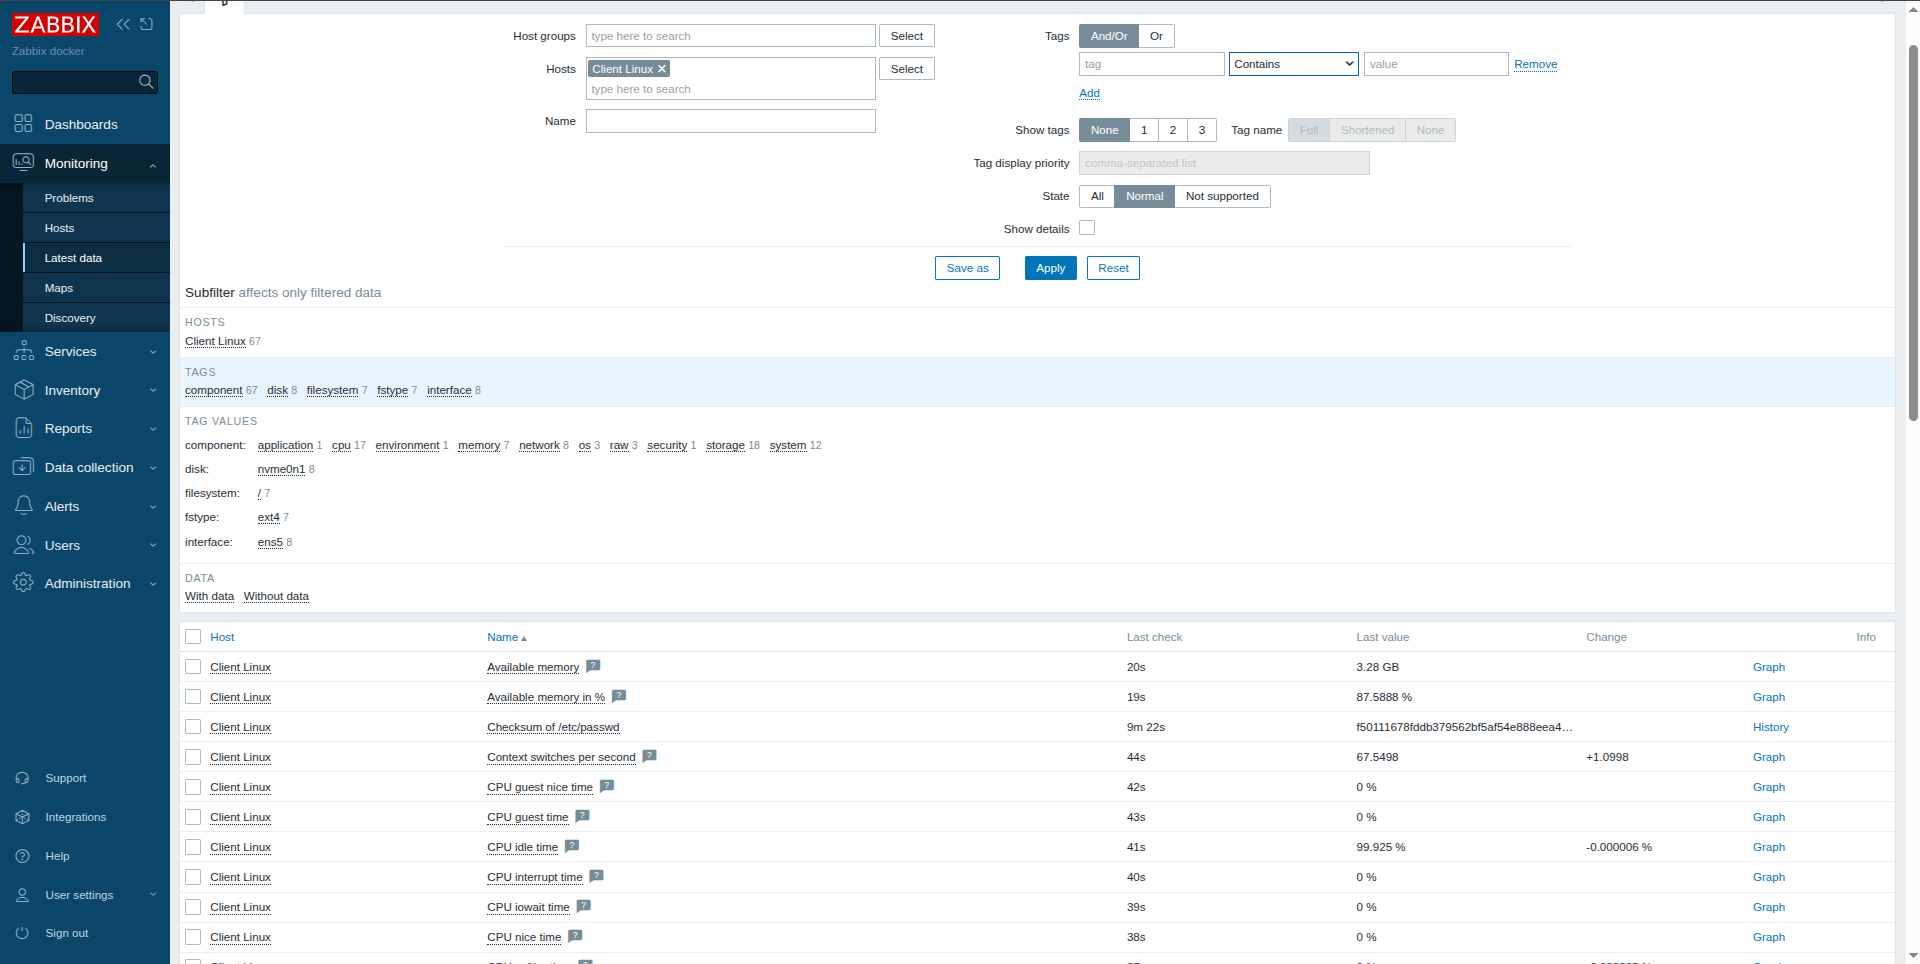
\includegraphics[width=0.95\textwidth]{images/29-zabbix-monitoring-problems.png}
\caption{Vue des problèmes actifs dans Zabbix}
\label{fig:monitoring-problems}
\end{figure}

\subsection{Liste des Problèmes}

\begin{figure}[H]
\centering
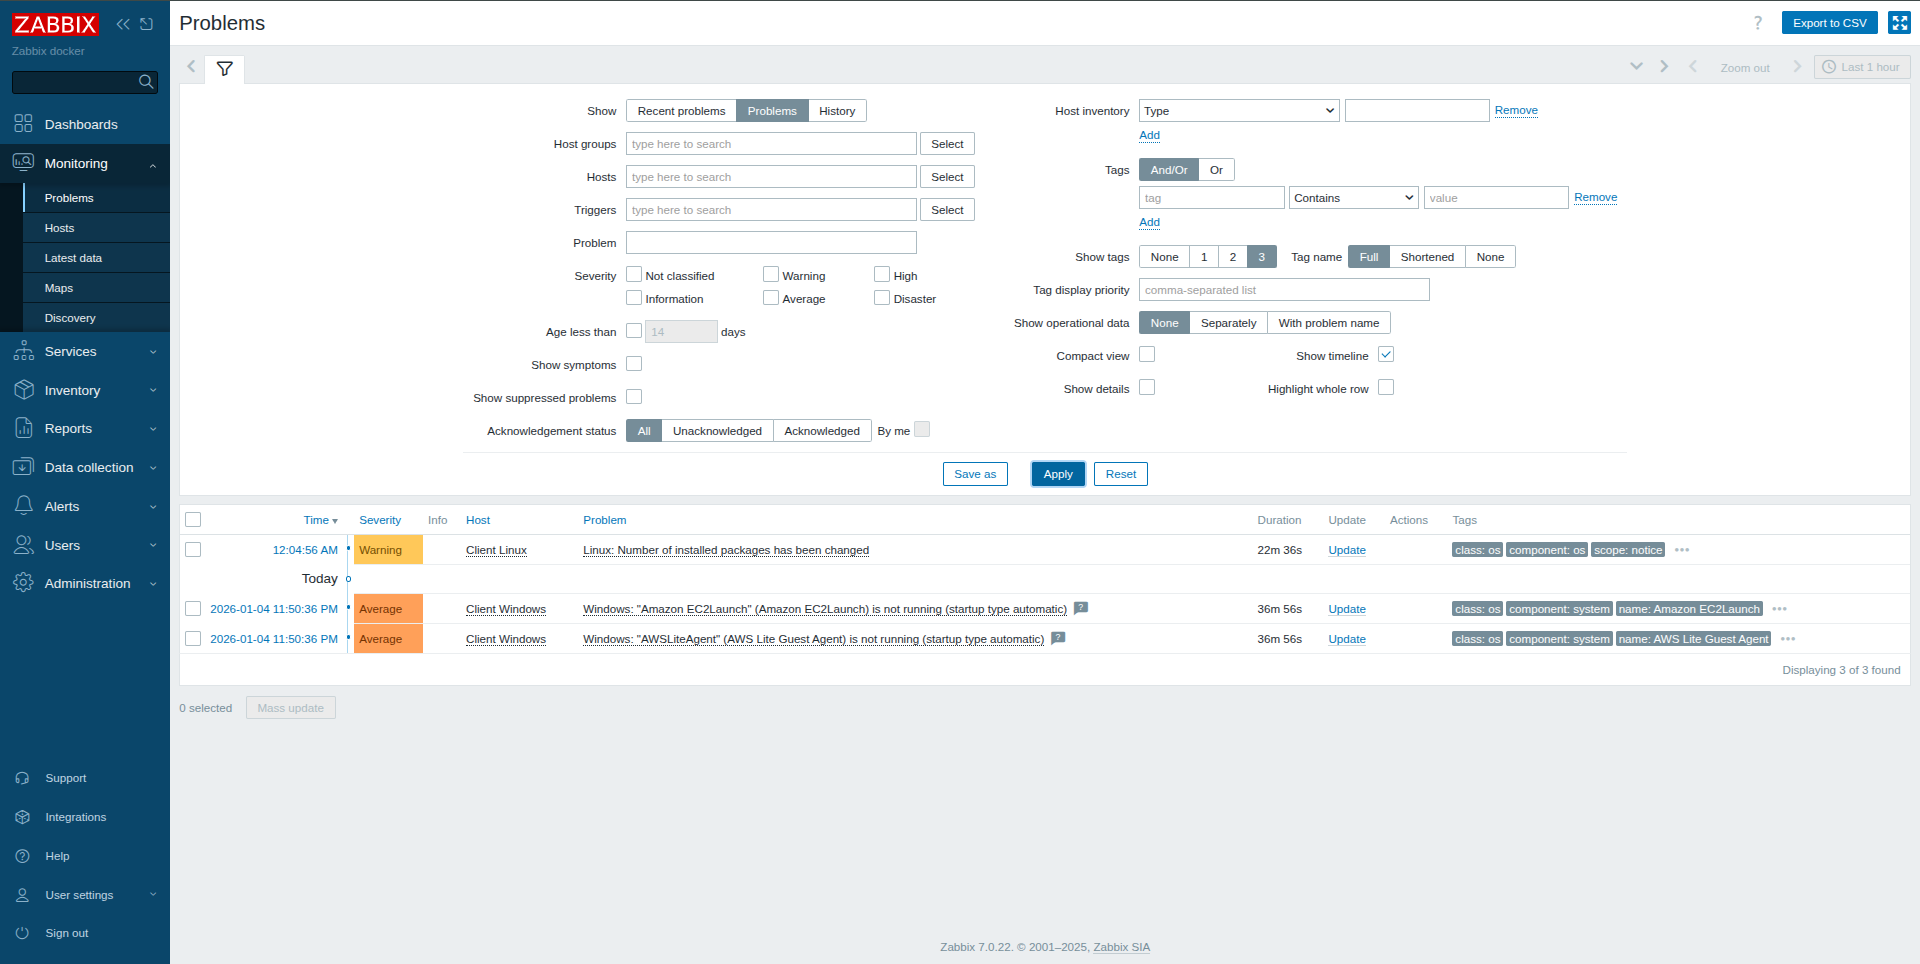
\includegraphics[width=0.95\textwidth]{images/30-zabbix-problems-list.png}
\caption{Liste détaillée des problèmes}
\label{fig:problems-list}
\end{figure}

\subsection{Historique des Événements}

L'historique complet des événements est disponible :

\begin{figure}[H]
\centering
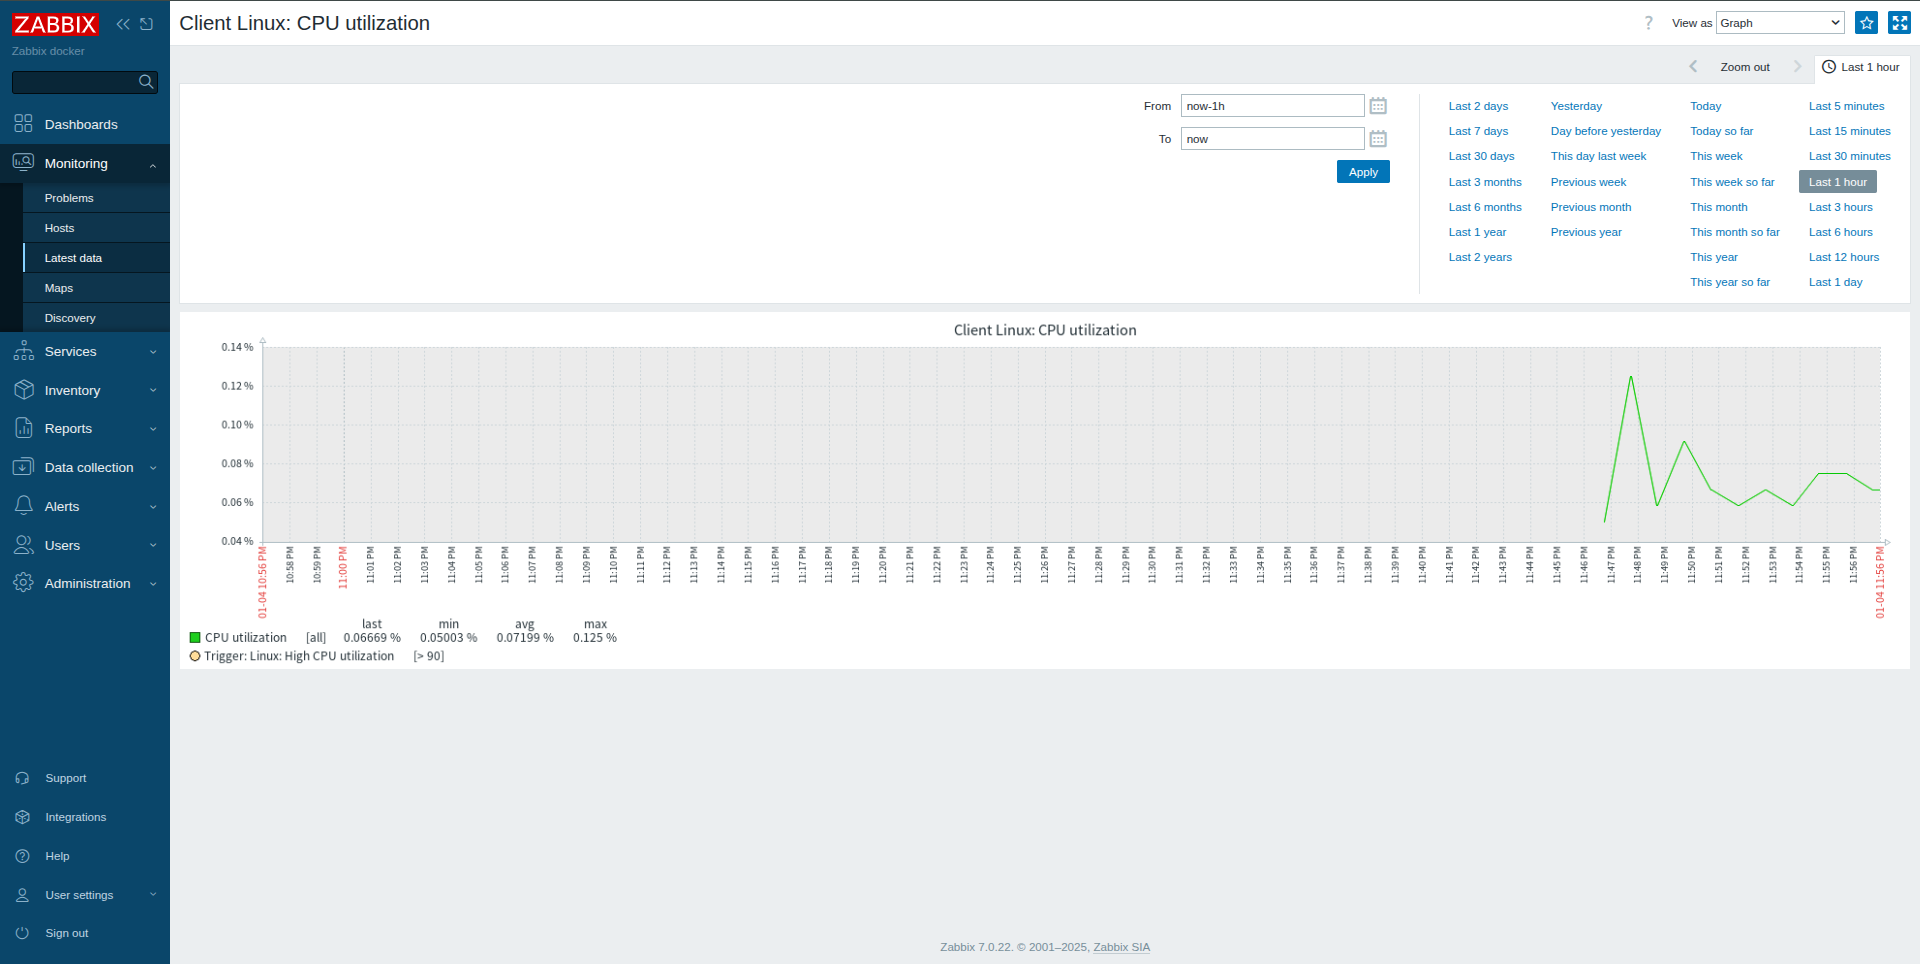
\includegraphics[width=0.95\textwidth]{images/31-zabbix-events-history.png}
\caption{Historique des événements Zabbix}
\label{fig:events-history}
\end{figure}

\section{Configuration des Triggers}

\subsection{Liste des Triggers}

Les triggers définissent les conditions de déclenchement des alertes :

\begin{figure}[H]
\centering
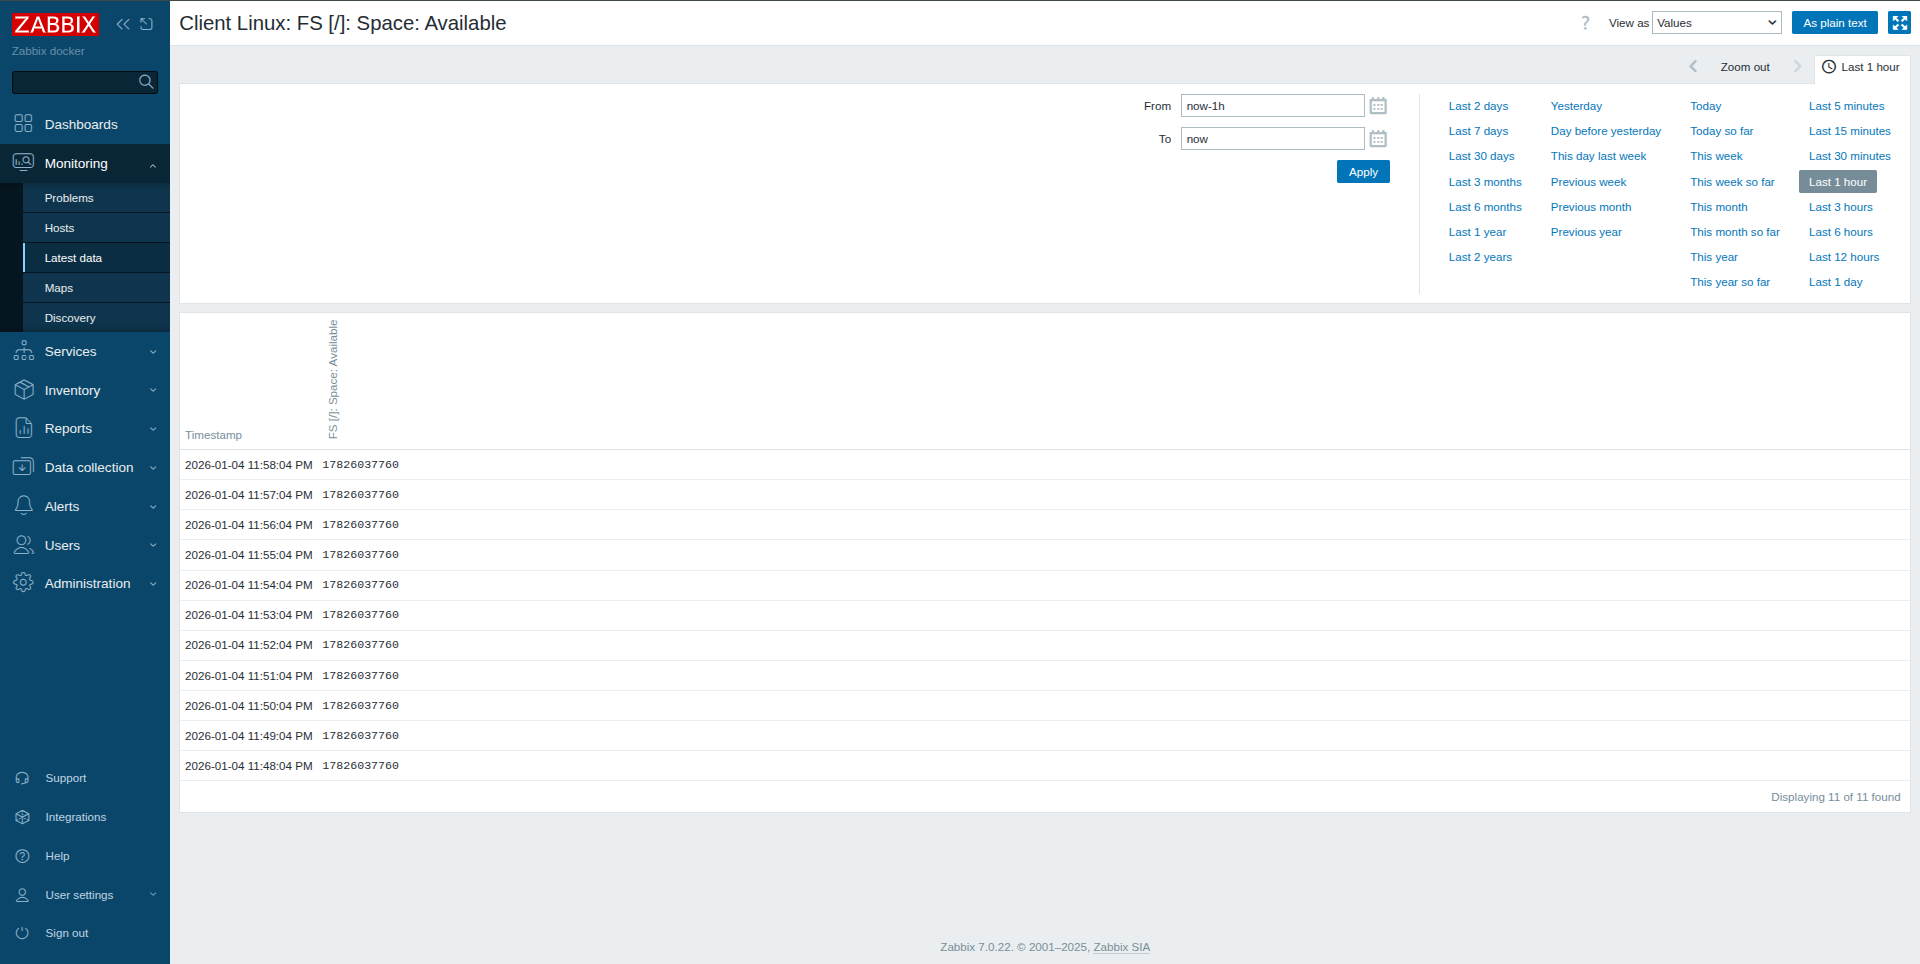
\includegraphics[width=0.95\textwidth]{images/32-zabbix-triggers-list.png}
\caption{Liste des triggers configurés}
\label{fig:triggers-list}
\end{figure}

\subsection{Exemples de Triggers}

\begin{table}[H]
\centering
\caption{Exemples de triggers Zabbix}
\label{tab:triggers-examples}
\begin{tabular}{|l|l|l|}
\hline
\textbf{Trigger} & \textbf{Sévérité} & \textbf{Condition} \\
\hline
High CPU utilization & Warning & CPU > 80\% pendant 5 min \\
\hline
High memory utilization & Warning & RAM > 90\% \\
\hline
Disk space critical & High & Espace disque < 10\% \\
\hline
Agent unreachable & Disaster & Pas de réponse pendant 3 min \\
\hline
\end{tabular}
\end{table}

\begin{figure}[H]
\centering
\includegraphics[width=0.95\textwidth]{images/33-zabbix-triggers-config.png}
\caption{Configuration d'un trigger}
\label{fig:triggers-config}
\end{figure}

\section{Visualisation des Données}

\subsection{Latest Data}

La section "Latest data" affiche les dernières valeurs collectées pour chaque métrique :

\begin{itemize}
    \item \textbf{Monitoring → Latest data}
    \item Filtrer par hôte ou groupe
    \item Voir les valeurs en temps réel
    \item Accéder aux graphiques historiques
\end{itemize}

\subsection{Graphiques}

Zabbix génère automatiquement des graphiques pour visualiser l'évolution des métriques dans le temps :

\begin{itemize}
    \item Graphiques CPU (utilisation, load)
    \item Graphiques mémoire (utilisée, libre)
    \item Graphiques réseau (trafic in/out)
    \item Graphiques disque (espace, I/O)
\end{itemize}

\section{Récapitulatif du Monitoring}

\begin{table}[H]
\centering
\caption{État final du monitoring}
\label{tab:monitoring-summary}
\begin{tabular}{|l|c|c|c|}
\hline
\textbf{Hôte} & \textbf{Statut} & \textbf{Template} & \textbf{Items} \\
\hline
Zabbix-Server & \textcolor{green}{ZBX} & Linux by Zabbix agent & ~150 \\
\hline
ELBadry-Client-Linux & \textcolor{green}{ZBX} & Linux by Zabbix agent & ~150 \\
\hline
ELBadry-Client-Windows & \textcolor{green}{ZBX} & Windows by Zabbix agent & ~200 \\
\hline
\end{tabular}
\end{table}

\section{Points Clés}

\begin{itemize}
    \item[$\checkmark$] Les 3 hôtes sont supervisés avec succès (ZBX vert)
    \item[$\checkmark$] Les métriques sont collectées en temps réel
    \item[$\checkmark$] Le stress test a déclenché les alertes appropriées
    \item[$\checkmark$] Les graphiques affichent l'historique des performances
    \item[$\checkmark$] Les triggers fonctionnent correctement
\end{itemize}

% ============================================
% Chapitre 7 : Conclusion
% ============================================
\chapter{Conclusion}
\label{chap:conclusion}

\section{Synthèse du Projet}

Ce projet a permis de mettre en œuvre avec succès une \textbf{infrastructure cloud de supervision centralisée} sur AWS. L'ensemble des objectifs fixés ont été atteints :

\begin{table}[H]
\centering
\caption{Objectifs atteints}
\label{tab:objectives-achieved}
\begin{tabular}{|l|c|}
\hline
\textbf{Objectif} & \textbf{Statut} \\
\hline
Création du VPC et de l'infrastructure réseau & $\checkmark$ \\
\hline
Déploiement de 3 instances EC2 & $\checkmark$ \\
\hline
Installation de Docker sur le serveur & $\checkmark$ \\
\hline
Déploiement de Zabbix conteneurisé & $\checkmark$ \\
\hline
Configuration de l'agent Linux & $\checkmark$ \\
\hline
Configuration de l'agent Windows & $\checkmark$ \\
\hline
Monitoring opérationnel (ZBX vert) & $\checkmark$ \\
\hline
Test d'alertes fonctionnel & $\checkmark$ \\
\hline
\end{tabular}
\end{table}

\section{Compétences Acquises}

\subsection{Amazon Web Services}

\begin{itemize}
    \item Configuration de VPC, subnets et Internet Gateway
    \item Gestion des Security Groups et règles de pare-feu
    \item Déploiement et gestion d'instances EC2
    \item Utilisation des différents types d'AMI (Ubuntu, Windows Server)
    \item Connexion SSH et RDP aux instances
\end{itemize}

\subsection{Docker et Conteneurisation}

\begin{itemize}
    \item Installation et configuration de Docker Engine
    \item Rédaction de fichiers docker-compose.yml
    \item Gestion des conteneurs, volumes et réseaux Docker
    \item Déploiement d'applications multi-conteneurs
\end{itemize}

\subsection{Zabbix et Monitoring}

\begin{itemize}
    \item Architecture serveur/agent de Zabbix
    \item Configuration des agents Linux et Windows
    \item Utilisation des templates de monitoring
    \item Configuration des triggers et alertes
    \item Interprétation des métriques et graphiques
\end{itemize}

\section{Difficultés Rencontrées}

\subsection{Problèmes et Solutions}

\begin{table}[H]
\centering
\caption{Difficultés et solutions apportées}
\label{tab:difficulties}
\begin{tabular}{|p{5.5cm}|p{8cm}|}
\hline
\textbf{Difficulté} & \textbf{Solution} \\
\hline
Temps de démarrage des conteneurs MySQL & Utilisation de healthcheck et depends\_on dans docker-compose \\
\hline
Communication agent/serveur bloquée & Vérification des Security Groups et ouverture du port 10050 \\
\hline
Pare-feu Windows bloquant l'agent & Création d'une règle entrante pour le port 10050 \\
\hline
Session Learner Lab expirée & Redémarrage des conteneurs avec docker compose up -d \\
\hline
Récupération du mot de passe Windows & Utilisation de la fonction "Get Windows Password" avec la clé PEM \\
\hline
\end{tabular}
\end{table}

\section{Limitations du Learner Lab}

Durant ce projet, plusieurs limitations du Learner Lab AWS Academy ont été identifiées :

\begin{itemize}
    \item \textbf{Types d'instances} : Limités à t3.medium et t3.large
    \item \textbf{Région} : Obligatoirement us-east-1 (N. Virginia)
    \item \textbf{Budget} : Limité à environ 50\$ de crédits
    \item \textbf{Sessions} : Arrêt automatique après un certain temps d'inactivité
    \item \textbf{Services} : Certains services AWS avancés non disponibles
\end{itemize}

\section{Améliorations Possibles}

Pour aller plus loin, plusieurs améliorations pourraient être apportées :

\begin{enumerate}
    \item \textbf{Haute disponibilité} : Déployer Zabbix en cluster avec réplication
    \item \textbf{HTTPS} : Configurer un certificat SSL pour l'interface web
    \item \textbf{Notifications} : Configurer les alertes par email ou Slack
    \item \textbf{Automatisation} : Utiliser Terraform pour l'infrastructure as code
    \item \textbf{Monitoring avancé} : Ajouter la supervision d'applications (MySQL, Nginx)
    \item \textbf{Dashboards personnalisés} : Créer des tableaux de bord adaptés aux besoins
\end{enumerate}

\section{Perspectives}

Ce projet constitue une base solide pour :

\begin{itemize}
    \item La mise en place de solutions de monitoring en entreprise
    \item L'apprentissage approfondi des services AWS
    \item La maîtrise de Docker et de l'orchestration de conteneurs
    \item La préparation aux certifications AWS et DevOps
\end{itemize}

\section{Conclusion Générale}

La réalisation de ce projet a permis d'acquérir une expérience pratique significative dans le domaine du cloud computing et du monitoring d'infrastructure. L'utilisation combinée d'AWS, Docker et Zabbix offre une solution robuste et évolutive pour la supervision d'environnements hybrides.

\vspace{1cm}

\begin{center}
\fbox{\parbox{0.8\textwidth}{
\centering
\textbf{Ressources du Projet}\\[0.3cm]
Dépôt GitHub : \url{https://github.com/VOTRE-USERNAME/aws-zabbix-monitoring}\\[0.2cm]
Documentation complète disponible dans le README
}}
\end{center}


\end{document}